\documentclass[12pt,german,a4paper,oneside,notitlepage]{report}



\usepackage{acronym} %Abk�rzungen
\usepackage{array}
\usepackage{cite} % Zitate
\usepackage[a4paper]{geometry} %Papiergroesse
\geometry{verbose,tmargin=2.5cm,bmargin=4.5cm,lmargin=2.5cm,rmargin=2.5cm}
\usepackage{fancyhdr}
\usepackage{graphicx}
\usepackage{listings}
\usepackage[ngerman]{babel} %Spracherg�nzung
\usepackage{picins}
\usepackage[intoc]{nomencl}
\usepackage[latin1]{inputenc}
\usepackage{setspace}
\usepackage{lastpage}
\usepackage[plainpages=false]{hyperref}

\usepackage{color}
\definecolor{lightgray}{rgb}{0.95, 0.95, 0.95}
\definecolor{darkgray}{rgb}{0.4, 0.4, 0.4}
%\definecolor{purple}{rgb}{0.65, 0.12, 0.82}
\definecolor{editorGray}{rgb}{0.95, 0.95, 0.95}
\definecolor{editorOcher}{rgb}{1, 0.5, 0} % #FF7F00 -> rgb(239, 169, 0)
\definecolor{editorGreen}{rgb}{0, 0.5, 0} % #007C00 -> rgb(0, 124, 0)
\definecolor{orange}{rgb}{1,0.45,0.13}      
\definecolor{olive}{rgb}{0.17,0.59,0.20}
\definecolor{brown}{rgb}{0.69,0.31,0.31}
\definecolor{purple}{rgb}{0.38,0.18,0.81}
\definecolor{lightblue}{rgb}{0.1,0.57,0.7}
\definecolor{lightred}{rgb}{1,0.4,0.5}


\setcounter{secnumdepth}{3}
\setcounter{tocdepth}{3}
\fontsize{12}{0}



\makeatletter 
\renewcommand\chapter{\@startsection
	{chapter}{1}{0mm}%         % name, ebene, einzug
	{.5\baselineskip}%            % vor-abstand
	{1.5\baselineskip}%            % nach-abstand
	{\bfseries\sffamily\huge}%      % layout
} 
\makeatother

\makeatletter 
\renewcommand\section{\@startsection
	{section}{2}{0mm}%         % name, ebene, einzug
	{1.5\baselineskip}%            % vor-abstand
	{1.5\baselineskip}%            % nach-abstand
	{\bfseries\sffamily\Large}%      % layout
} 
\makeatother

\makeatletter 
\renewcommand\subsection{\@startsection
	{subsection}{3}{0mm}%         % name, ebene, einzug
	{.5em}%            % vor-abstand
	{.5em}%            % nach-abstand
	{\bfseries\sffamily\large}%      % layout
} 
\makeatother 

\makeatletter 
\renewcommand\subsubsection{\@startsection
	{subsubsection}{4}{0mm}%         % name, ebene, einzug
	{.5em}%            % vor-abstand
	{.5em}%            % nach-abstand
	{\bfseries\sffamily}%      % layout
} 
\makeatother 


\providecommand{\printnomenclature}{\printglossary}
\providecommand{\makenomenclature}{\makeglossary}
%f�r Abk Verz mit nomencl
\makenomenclature

\setlength{\headheight}{1.5cm}

\makeatletter

\providecommand{\tabularnewline}{\\}

\makeatother

\fancypagestyle{plain}{
	\fancyhf{}
	%	\renewcommand{\headrulewidth}{0.1pt}
	%	\renewcommand{\footrulewidth}{0.1pt}
	\fancyhead[L]{
		Studienarbeit
	}
	\fancyhead[R]{
		
\includegraphics[height=1cm]{images/dhbw}
	}
	\fancyfoot[L]{
		\noindent 
		{
			\begin{tabular*}{16cm}{@{\extracolsep{\fill}}l>{\raggedleft}p{8cm}}
				{\tiny Stand: \today} & {\tiny Seite \thepage~von~\pageref{LastPage}}\tabularnewline
			\end{tabular*}
		}
	}
}
\pagestyle{plain}

\renewcommand{\nomname}{Abk�rzungsverzeichnis}

\newcounter{alteSeitenzahl}




%----------------------------------------------------------
\begin{document}
	\pagenumbering{roman}
	
	
	
	
	\singlespace
	\pagestyle{plain}
	\pagenumbering{arabic}

	\tableofcontents{}
	\newpage
	
	
	\chapter*{Abk�rzungsverzeichnis}
	\addcontentsline{toc}{chapter}{Abk�rzungsverzeichnis}
	\begin{acronym}
		\acro{zb}{zum BSP}
		\acro{3D}{dreidimensional}
		\acro{DHBW}{Duale Hochschule Baden-W�rttemberg}
	\end{acronym}
		
	TEST\ac{zb}    TEST \ac{zb}
	
	
	
	\newpage{}
	\begingroup
	\onehalfspacing
	\setlength{\parskip}{1.5ex}
	
	
	
	
	%--------------CHAPTER----------------
	
	\chapter{Einleitung}
	\chapter{Einleitung}

Bei herk�mmlichen Verfahren, um Objekte aus Grundstoffen wie beispielsweise Metallen, Kunststoffen oder Harzen anzufertigen, werden diese oft subtraktiv aus einem gro�en Block des Grundstoff herausgearbeitet. Dies kann beispielsweise durch Fr�sen erfolgen. 


Neben diesen Verfahren gibt es auch die sogenannten additiven Verfahren, bei denen ein Objekt nach und nach (meist schichtweise) aus dem Grundstoff hergestellt wird. Die Vorteile dieser Verfahren sind unter anderem, dass weniger Material verbraucht wird und auch komplexere Formen relativ einfach realisiert werden k�nnen. \\
Einige dieser Verfahren werden in der Industrie bereits verwendet, beispielsweise um medizinische Implantate herzustellen. \\
Ein gro�es Anwendungsgebiet liegt im Bereich des Rapid Prototyping. Dabei geht es darum, m�glichst schnell Prototypen herzustellen, beispielsweise um die Eignung eines Designs f�r das sp�tere Serienprodukt zu erforschen. Da hier nur geringe St�ckzahlen ben�tigt werden und m�glichst keine komplizierten Serienwerkzeuge hergestellt werden sollen, eignen sich additive Verfahren gut f�r diese Anwendung.


In den letzten Jahren wird zunehmend auch der Endkundenmarkt erschlossen. Sogenannte \ac{3D}-Drucker, die in der Regel auf dem Extrusionsverfahren basieren, werden inzwischen zu erschwinglichen Preisen angeboten.

 
Im letzten Jahr hat die \ac{DHBW} einen solchen \ac{3D}-Drucker, den Ultimaker 2, angeschafft. In einer vorigen Studienarbeit wurde dieser in Betrieb genommen und erste Objekte gedruckt.
 
In dieser Studienarbeit soll weiter mit dem Drucker gearbeitet werden.
 
Das Ziel dieser Studienarbeit ist es, mithilfe verschiedener Programme ein technisches und ein organisches Objekt zu erstellen. Anschlie�end sollen diese mit dem Ultimaker 2 gedruckt werden. 
Die dabei gewonnenen Erkenntnisse sollen auf einer bereits existierenden Website �ber den \ac{3D}-Drucker dokumentiert werden. 
 
Dieser Bericht wird zun�chst einen �berblick �ber verschiedene verbreitete additive Verfahren geben. Anschlie�end werden der Ultimaker 2, die dazugeh�rige Toolchain sowie die verwendeten \ac{CAD} Programme n�her erl�utert.
 
Basierend auf diesen Grundlagen wird dann im Hauptteil des Berichts die Erstellung des technischen und organischen Objekts n�her beschrieben. 
	\chapter{Stand der Technik}
	%m�gliche Techniken
	\chapter{ultimaker}
		\chapter{ultimaker}
	\chapter{Entwicklung eines technischen Objekts}
		\chapter{Entwicklung eines technischen Objekts}
\label{chapter:techObj}

% explizite Bezug auf Ultimaker 2, andere Drucker liefern andere Ergebnisse

Dieses Kapitel handelt vom Entwurf und Druck eines technischen Objekts. Ein technisches Objekt wird dabei als ein Objekt definiert, das entwickelt wird, um einen bestimmten technischen Zweck zu erf�llen und in erster Linie funktional sein soll. Eine ansprechende oder dekorative Optik des Objekts ist deshalb unwichtig oder zumindest zweitrangig. Wichtig ist hingegen, dass ein solches Objekt m�glichst einfach zu produzieren ist. Technische Objekte besitzen beispielsweise meist glatte Oberfl�chen, da diese wesentlich einfacher und genauer zu produzieren sind als gew�lbte Oberfl�chen. Zudem muss das Objekt fest definierte Ma�e besitzen. 

Bei der Produktion eines technischen Objekts ist es wichtig, dass diese Ma�e mit m�glichst geringen Toleranzen eingehalten werden. Wird mehrfach dasselbe Objekt mit denselben Werkzeugen und Prozessen hergestellt, sollten die Ergebnisse vergleichbar sein.  \\

F�r diese Studienarbeit wird als technisches Objekt exemplarisch ein Aufbewahrungssystem f�r einen Raspberry Pi, der mit einem \ac{USB}- Hub und einer externen Festplatte gekoppelt ist, entworfen. Dieses System soll m�glichst kompakt und als ein Block transportierbar sein.

Diese Arbeit bezieht sich h�ufig auf den Ultimaker 2, der im vorhergehenden Kapitel \ref{chapter:techGr:ultimaker2} vorgestellt wird. In der Arbeit mit einem anderen Drucker k�nnen sich Vorgehensweise und Ergebnis deutlich unterscheiden.

In diesem Kapitel wird zuerst das bestehende Aufbewahrungssystem analysiert. Anschlie�end folgt eine Beschreibung des Konzepts f�r das neue Aufbewahrungssystem, das w�hrend der Studienarbeit gedruckt werden soll. Folgend werden der Entwurf des Systems mit einem \ac{CAD}-Programm  und der Druck des Objekts beschrieben. Zuletzt folgt ein Fazit �ber die Eignung des Ultimaker 2 zum Drucken von technischen Objekten.


%%TODO Ist-Analyse
\newpage
\section{Ist-Analyse}
	Zu entwerfen ist ein Aufbewahrungssystem f�r einen Heimserver auf einem Raspberry Pi(folgend als Pi bezeichnet) mit angeschlossener externer Festplatte. Der Pi selbst liefert an seinen \ac{USB}-Ports nicht genug Leistung zum Betreiben der Festplatte, weshalb ein zus�tzlicher powered \ac{USB}-Hub n�tig ist. 
	
	\piccaption{Urspr�ngliches Stapelsystem\label{grafik:techObj:ursprStapelsystem}}
	\parpic[r]{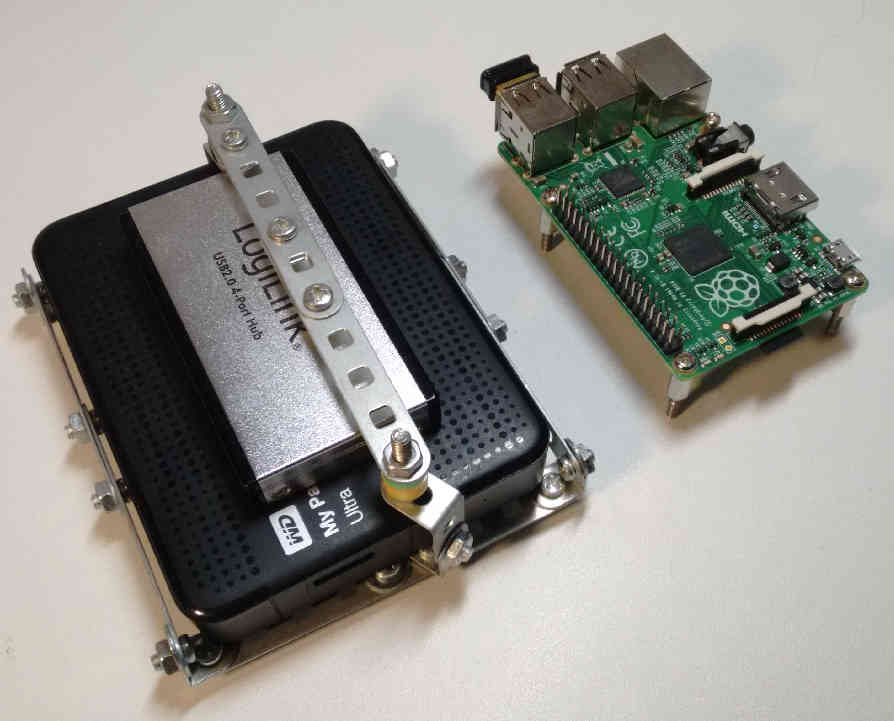
\includegraphics[width=.5\textwidth]{images/techObj/urspruenglicheHalterung02.jpg}}
	
	Zu Beginn der Entwicklung wurde das System durch zu einem K�fig verschraubte Lochbleche zusammengehalten, die Festplatte und Hub umfassten, wie in Abbildung \ref{grafik:techObj:ursprStapelsystem} zu sehen ist. Insbesondere der Pi war im alten System nur unzureichend fixiert, da er nur auf den K�fig aufgesetzt wurde. Eine Hauptanforderung an das neue System soll deshalb das sichere Lagern aller Komponenten sein. 
	
	\picskip{0}
	\vspace*{4em}
	
	Die zweite Anforderung ist die Portabilit�t des Systems. Um den Server sicher und einfach bewegen zu k�nnen, soll das System als Ganzes stabil zu einer Einheit verbunden werden k�nnen. Das bisherige System sollte die Portabilit�t erm�glichen, war jedoch aufgrund der oben genannten Instabilit�t dazu nicht in der Lage.  
	
	
	%TODO Messung Dimensionen
%	\begin{tabular}{c|c|c|c}
%		\label{}
%		\caption{�bersicht der Dimensionen der einzubauenden Objekte}
%				Bauteil 			& L�nge [mm] 	& Breite [mm]	& H�he [mm] \\ 
%		\hline 	Raspberry Pi 		& 85 	& 56 	& 17  \\ 
%				externe Festplatte 	& 111 	& 83,5 	& 21  \\ 
%				\ac{USB}-Hub 		& 42,2 	& 77,6 	& 11,7  \\ 
%		 
%	\end{tabular} 

	Die Ausma�e der zu verstauenden Objekte sind in Abbildung \ref{figure:techObj:bemassungIstAnalyse} zu sehen.
	
	\begin{figure}[h!]
		
		
		\begin{minipage}[b]{.3\textwidth}
			
			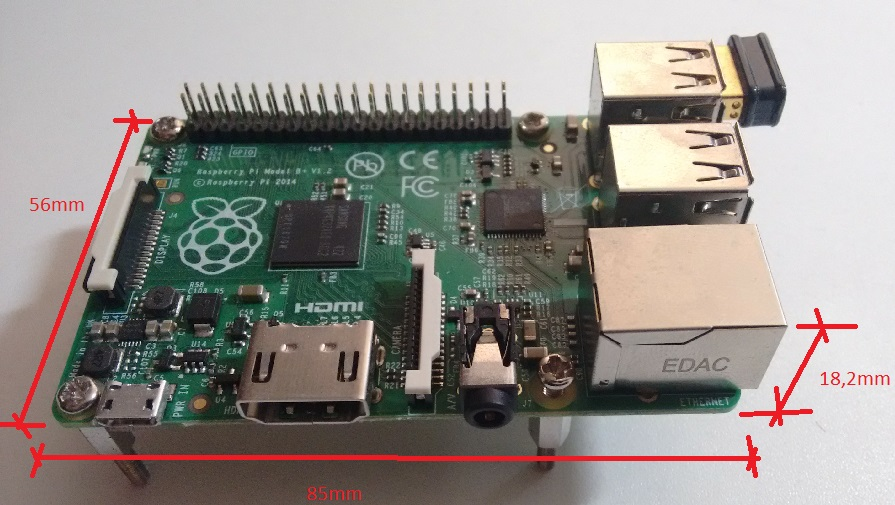
\includegraphics[width=\textwidth]{images/techObj/pi/raspberry_bemasst}
			\subcaption{Bema�ung des Raspberry Pi}
			
		\end{minipage}
		\begin{minipage}[b]{.3\textwidth}
			
			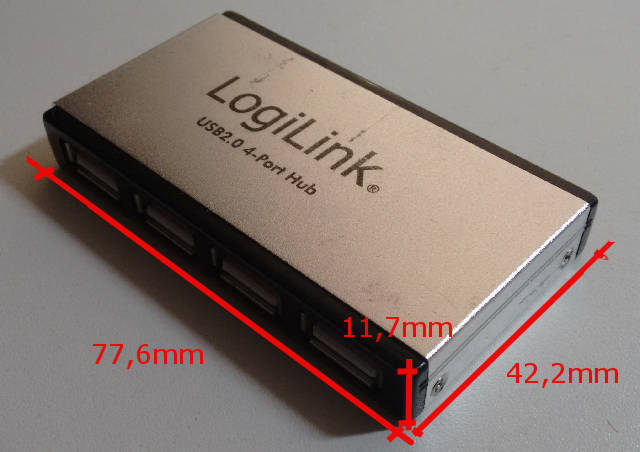
\includegraphics[width=\textwidth]{images/techObj/Hub/Hub_bemasst.jpg}
			\subcaption{Bema�ung des \ac{USB}-Hubs}
			
		\end{minipage}
		\begin{minipage}[b]{.3\textwidth}
			
			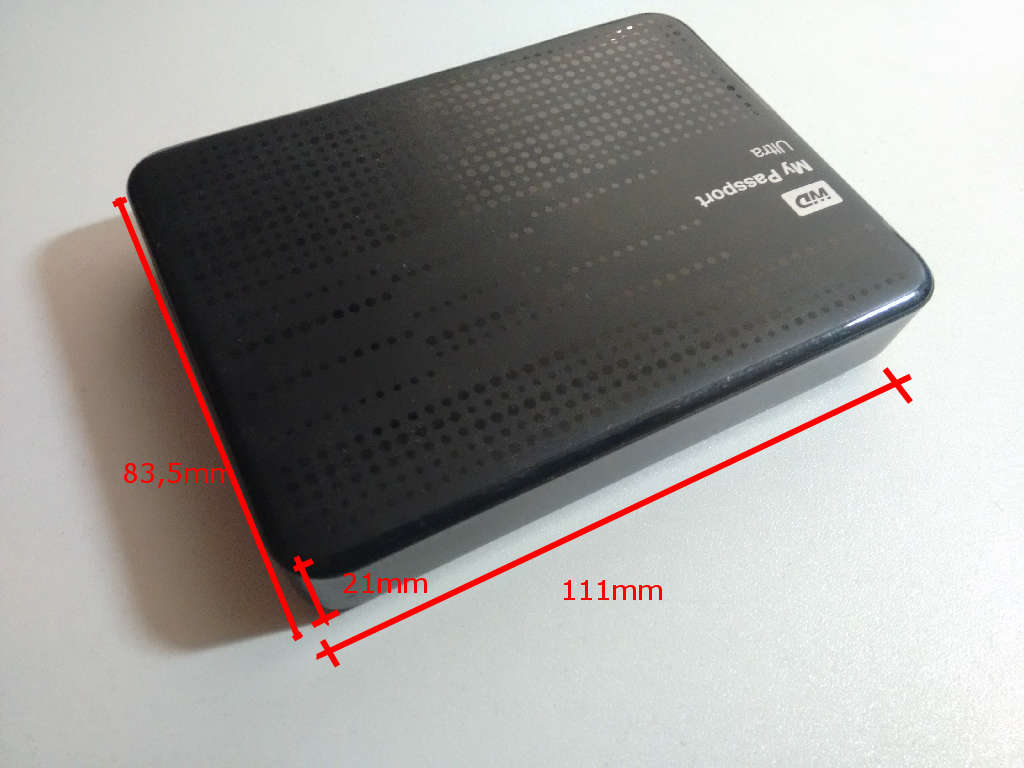
\includegraphics[width=\textwidth]{images/techObj/FP/FP_bemasst.jpg}
			\subcaption{Bema�ung der externen Festplatte}
			
		\end{minipage}
		\label{figure:techObj:bemassungIstAnalyse}
		\caption{Bema�ung der einzufassenden Objekte}
	\end{figure}
	

	Zus�tzlich zu diesen Ma�en kommen beim Pi noch die Positionen der Schraubbohrungen und die H�he der unter dem Pi herausragenden L�tpunkte und \ac{SMD}-Bauteile hinzu. Die frei zug�nglichen Leiterbahnen m�ssen in der Verwahrung genug Abstand zu anderen Bauteilen haben, da sie sonst besch�digt werden k�nnten.
	
	Eine Eigenschaft des bisherigen Systems mit den Lochblechen soll f�r das neue Aufbewahrungssystem �bernommen werden. Die Platzierung der Komponenten �bereinander ist sehr platzsparend. Zudem kann das System dadurch gut transportiert werden.

	
%%TODO 
\section{Konzept: Modulare Boxen}
	Als Ersatz f�r den oben beschriebenen K�fig aus Lochblechen soll ein modulares Stapelsystem dienen. Auf einer massiven Grundplatte werden Boxen gestapelt. Jede Box beinhaltet eine Komponente (Raspberry Pi, \ac{USB}-Hub oder Festplatte). Die Au�enma�e der Boxen sind in Breite und L�nge immer gleich. Diese Grundfl�che wird durch die gr��te zu befestigende Komponente, hier also die Festplatte, bestimmt. Der Innenraum einer Box ist an die jeweilige Komponente angepasst. Abh�ngig von der Komponente werden verschiedene Aussparungen in den Seitenw�nden der Boxen angebracht, durch die Kabel gef�hrt werden k�nnen. Im Aufbewahrungssystem werden die Boxen auf der Grundplatte gestapelt.
	
	Um das Aufbewahrungssystem zusammenzuhalten, werden Rahmen zwischen die Boxen gelegt, die die Boxen zwischen Gewindestangen fixieren. Die Gewindestangen sind an der Unterseite der Grundplatte festgeschraubt. Dadurch ist das Stapelsystem im Ganzen stabilisiert und kann problemlos transportiert werden. 
	
	Das System ist zudem einfach um neue Komponenten erweiterbar, sofern diese von der Grundfl�che her nicht gr��er sind als die Grundfl�che der Boxen. F�r neue Komponenten kann eine eigene Box mit den passenden Au�enma�en und angepasstem Innenraum und H�he designt werden. Diese Box kann dann wie beschrieben mit Rahmen am System befestigt werden.



\section{Entwurf}

	
	\begin{figure}[h!]
		\begin{minipage}{.26\textwidth}
			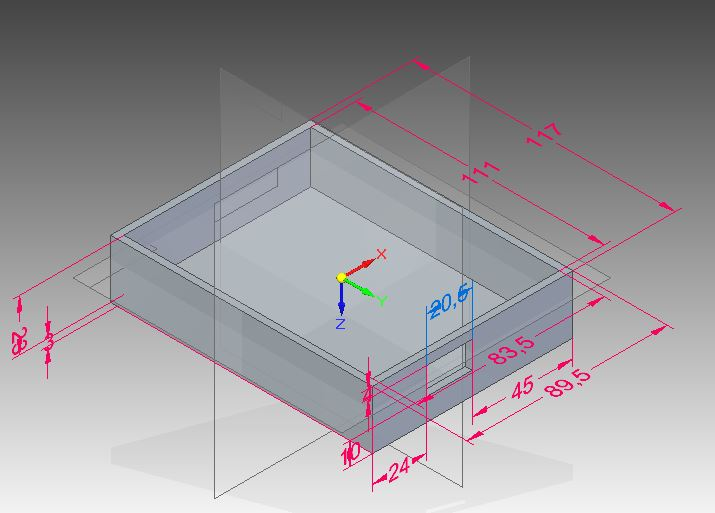
\includegraphics[height=7em]{images/techObj/entwurf/FPBox}
			\subcaption{Festplattenbox}
			\label{figure:techObj:entwurf:fpbox}
		\end{minipage}
		\begin{minipage}{.3\textwidth}
			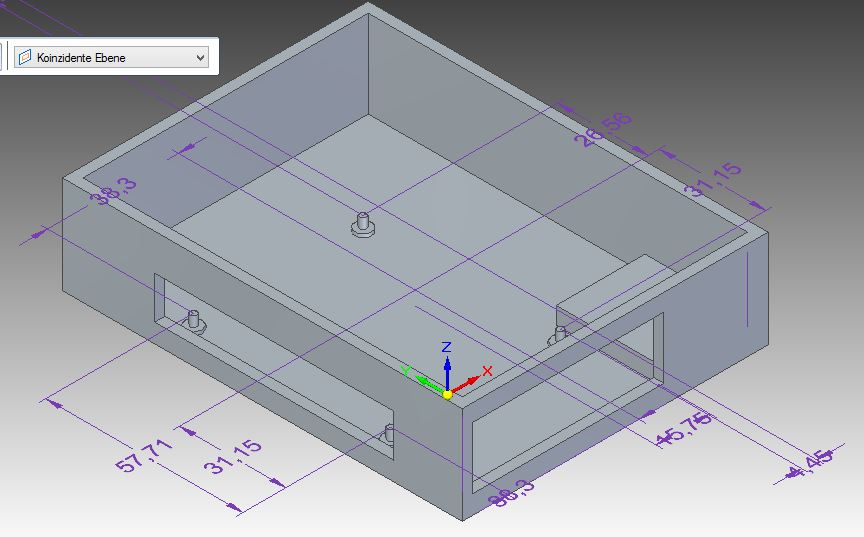
\includegraphics[height=7em]{images/techObj/entwurf/PiBox}
			\subcaption{Pi-Box}
			\label{figure:techObj:entwurf:pibox}
		\end{minipage}
		\begin{minipage}{.34\textwidth}
			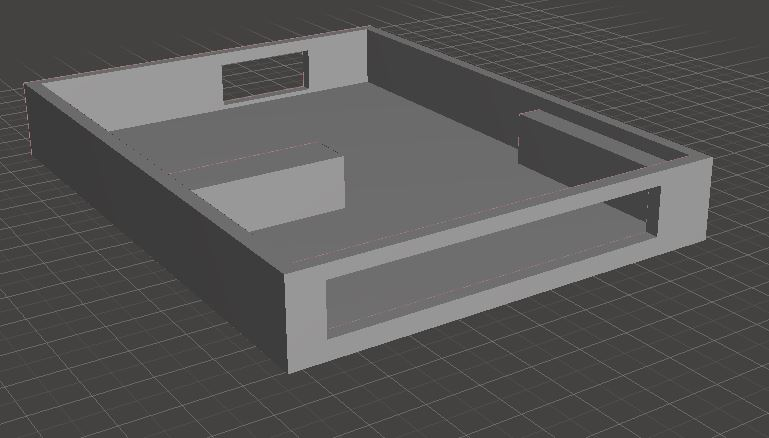
\includegraphics[height=7em]{images/techObj/entwurf/HubBox}
			\subcaption{Hub-Box}
			\label{figure:techObj:entwurf:hubbox}
		\end{minipage}
%		\caption{Entwurf der Objekte}
		
%	\end{figure}
%
%	\begin{figure}[h!]
		\begin{minipage}{.49\textwidth}
			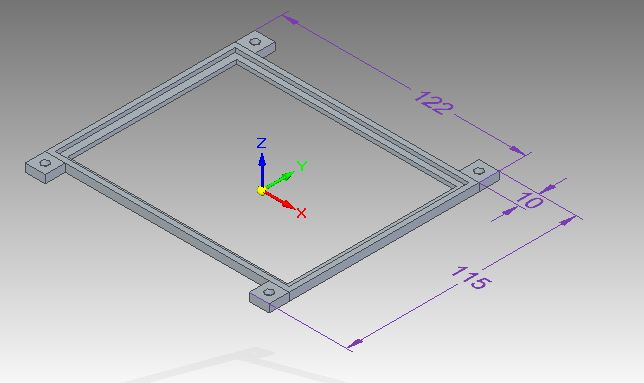
\includegraphics[height=11em]{images/techObj/entwurf/rahmen}
			\subcaption{Rahmen}
			\label{figure:techObj:entwurf:rahmen}
		\end{minipage}
		\begin{minipage}{.41\textwidth}
			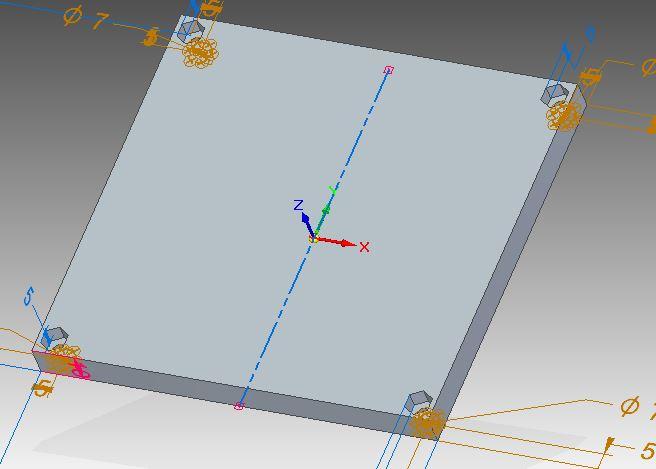
\includegraphics[height=11em]{images/techObj/entwurf/bodenplatte}
			\subcaption{Bodenplatte}
			\label{figure:techObj:entwurf:bodenplatte}
		\end{minipage}
		\caption{Entwurf der Objekte}
	\end{figure}
	Das Konzept soll f�r die vorhandenen Komponenten, also f�r Raspberry Pi, \ac{USB}-Hub und Festplatte, umgesetzt werden. Die zu druckenden Objekte werden mit dem \ac{CAD}-System Solid Edge designt. 
	
	
	Als erster Schritt werden die Ma�e von Festplatte, \ac{USB}-Hub und Raspberry Pi genommen. Davon ausgehend wird f�r jede Komponente eine Box entworfen.
	
	%Bild Ma�e, IST-ANALYSE?
	Die Ma�e definieren die Innengestaltung der jeweiligen Box. Die Grundfl�che ist durch die gr��te Box definiert, w�hrend die H�he der einzelnen Boxen pro Komponente festlegbar ist. Folgend werden die Designs der einzelnen Komponenten vorgestellt.
	
	%Bild FP-Box
	%TODO: Was f�r eine Schnittstelle?
	Die Festplatten-Box als einfachste und gr��te Komponente des Systems definiert die Au�enma�e und Form der quaderf�rmigen Boxen. An der Position der Schnittstelle ist ein Ausschnitt in Gr��e der Steckverbindung aus der Wand geschnitten. Da die Box einem gro�en Gewicht standhalten muss, wird eine Wandst�rke von 3mm gew�hlt. Abbildung \ref{figure:techObj:entwurf:fpbox} zeigt den Entwurf der Box.
	
	%Bild Hub-Box
	Da der \ac{USB}-Hub kleiner ist als die Festplatte, muss er auf der Grundfl�che der Box in Breite und Tiefe fixiert werden. Hierf�r werden seitlich und hinter den Hub Bl�cke gesetzt, die den Hub an der gew�nschten Position halten. Die Wand der Box ist wie bei der Festplattenbox auf H�he der Schnittstellen ausgeschnitten. Zus�tzlich gibt es einen Ausschnitt an der R�ckseite der Box, durch die Stromzufuhr und Anschlusskabel f�r den Raspberry Pi hinausgef�hrt werden k�nnen.
	Die Box ist in Abbildung \ref{figure:techObj:entwurf:hubbox} dargestellt.
	
	%Bild Raspberry
	Die Box f�r den Raspberry Pi erfordert einen gr��eren Design-Aufwand als die zuvor beschriebenen Boxen. Auf der Unterseite ben�tigt der Pi, aufgrund seiner L�tpunkte und \ac{SMD}-Bauteile, Abstand zum Boden. Daher wird er auf S�ulen gesetzt, die ihn in seinen Schraub-Bohrungen fixieren. Die zus�tzliche H�he, die dadurch entsteht, muss bei den Ausschnitten der Schnittstellen miteinbezogen werden. Damit alle Schnittstellen erreichbar sind, wird der Pi in eine Ecke der Box platziert.
	In Abbildung \ref{figure:techObj:entwurf:pibox} ist die Pi-Box dargestellt.
	
	%Bild Rahmen
	Um die Boxen gegen Verrutschen zu sichern, sind zwischen ihnen Rahmen platziert, die Einschnitte in Gr��e der Box-Grundfl�che haben. Zus�tzlich sind an jedem Rahmen vier runde Durchf�hrungen angebracht, mit denen sie auf einer Gewindestange eingef�delt werden k�nnen. Das vollst�ndige System kann dann durch vier M4-Muttern fixiert werden. Die Rahmen sind in der Fl�che nicht gef�llt; die Stabilit�t ist schon durch die eingeschlossenen Boxen gegeben. 
	Abbildung \ref{figure:techObj:entwurf:rahmen} zeigt den Entwurf des Rahmens.
	
	%Bild Bodenplatte
	Die Bodenplatte ist das Grundger�st des Systems. Da die Gewindestangen au�erhalb der Boxen durch die Durchf�hrungen in den Rahmen verlaufen, ist die Bodenplatte um die Gr��e der Durchf�hrungen breiter und l�nger als die Boxen. 
	An derselben Position wie die Rahmen hat auch die Bodenplatte Durchf�hrungen f�r die Gewindestangen. Die vier Gewindestangen werden durch die Bodenplatte gef�hrt und an der Unterseite der Bodenplatte mit M4-Muttern festgeschraubt. Damit das Aufbewahrungssystem nicht nur auf diesen vier Muttern steht, sind an der Unterseite der Bodenplatte Einschnitte f�r die M4-Muttern vorgesehen. Dadurch steht das Aufbewahrungssystem stabil auf der Bodenplatte.
	Der Entwurf der Bodenplatte ist in Abbildung \ref{figure:techObj:entwurf:bodenplatte} dargestellt.
	
\section{Druck des Objekts}
% Welche Parameter? --> spezifisch beim technischen Objekt
% Ver�nderungen durch Params?
%Parameter: Konzentrisch, Infill-dichte, Geschwindigkeit


Dadurch, dass das Aufbewahrungssystem aus vielen einzelnen Komponenten zusammengesetzt ist, sind auch viele Drucke notwendig. Einige der Komponenten, wie beispielsweise die Deckel f�r die Boxen und die Rahmen, werden zudem in mehrfacher Ausf�hrung ben�tigt. 
Dadurch ist insgesamt ein hoher Zeitaufwand mit dem Druck verbunden. 

Zus�tzlich zu der hohen Anzahl an Komponenten, die gedruckt werden m�ssen, kommt, dass einige Fehldrucke auftraten. Au�erdem zeigte sich beim Drucken der Komponenten, dass manche Ma�e aufgrund der Ungenauigkeit des Druckers zu gering gew�hlt waren und die Komponenten neu bema�t und gedruckt werden mussten. 

Im Folgenden wird der Druck der Komponenten kurz beschrieben und gegebenenfalls Besonderheiten beim Druck erw�hnt. Auf die Fehler, die beim Druck auftraten, wird an dieser Stelle nicht n�her eingegangen.
Die Fehler werden im Kapitel \ref{chapter:fehler} ausf�hrlicher beschrieben.

\subsection{Deckel}
\piccaption{Gedruckter Deckel \label{figure:techObj:druck:deckel}}
\parpic[r]{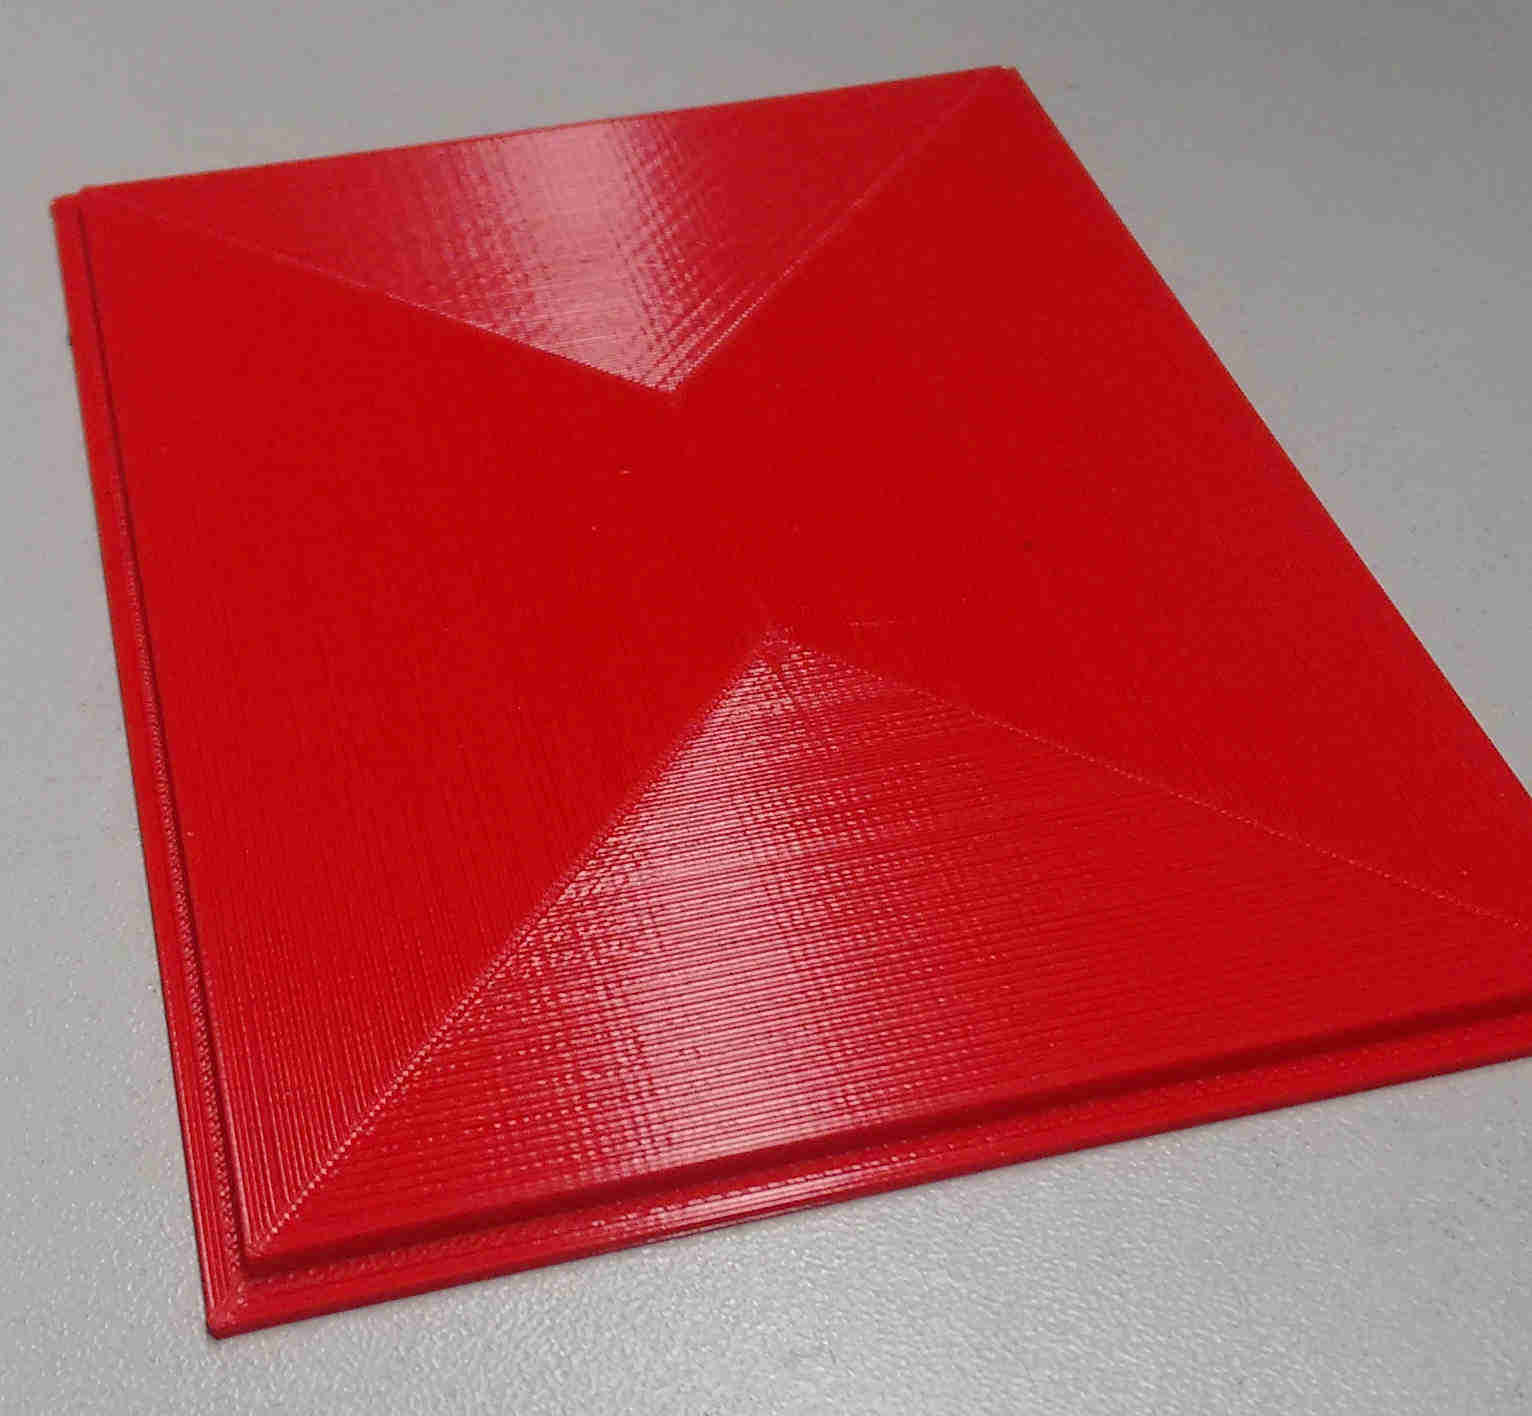
\includegraphics[width=.4\textwidth]{images/techObj/bilder/Deckel}}

Dadurch, dass der Deckel relativ d�nn ist, ist es wichtig zu gew�hrleisten, dass er dennoch stabil ist. Deshalb wird er massiv gedruckt. Aufgrund der geringen Gr��e dauert der Druck dennoch nicht unakzeptabel lange.

Wie in Abbildung \ref{figure:techObj:druck:deckel} zu sehen ist, wird der Deckel mit einem konzentrischen Infill-Pattern gedruckt. Dieses Muster kann vom Drucker schneller gedruckt werden als andere Muster und liefert gen�gend Stabilit�t f�r den Deckel. 

Es ist jedoch auff�llig, dass der Druck mit rotem Filament deutlich besser gelingt als mit durchsichtigem. Dieser Effekt wird in Kapitel \ref{chapter:fehler:material} n�her erl�utert.
\picskip{0}
\vspace*{3em}

\newpage

\subsection{Rahmen}

\piccaption{Gedruckter Rahmen \label{figure:techObj:druck:rahmen}}
\parpic[r]{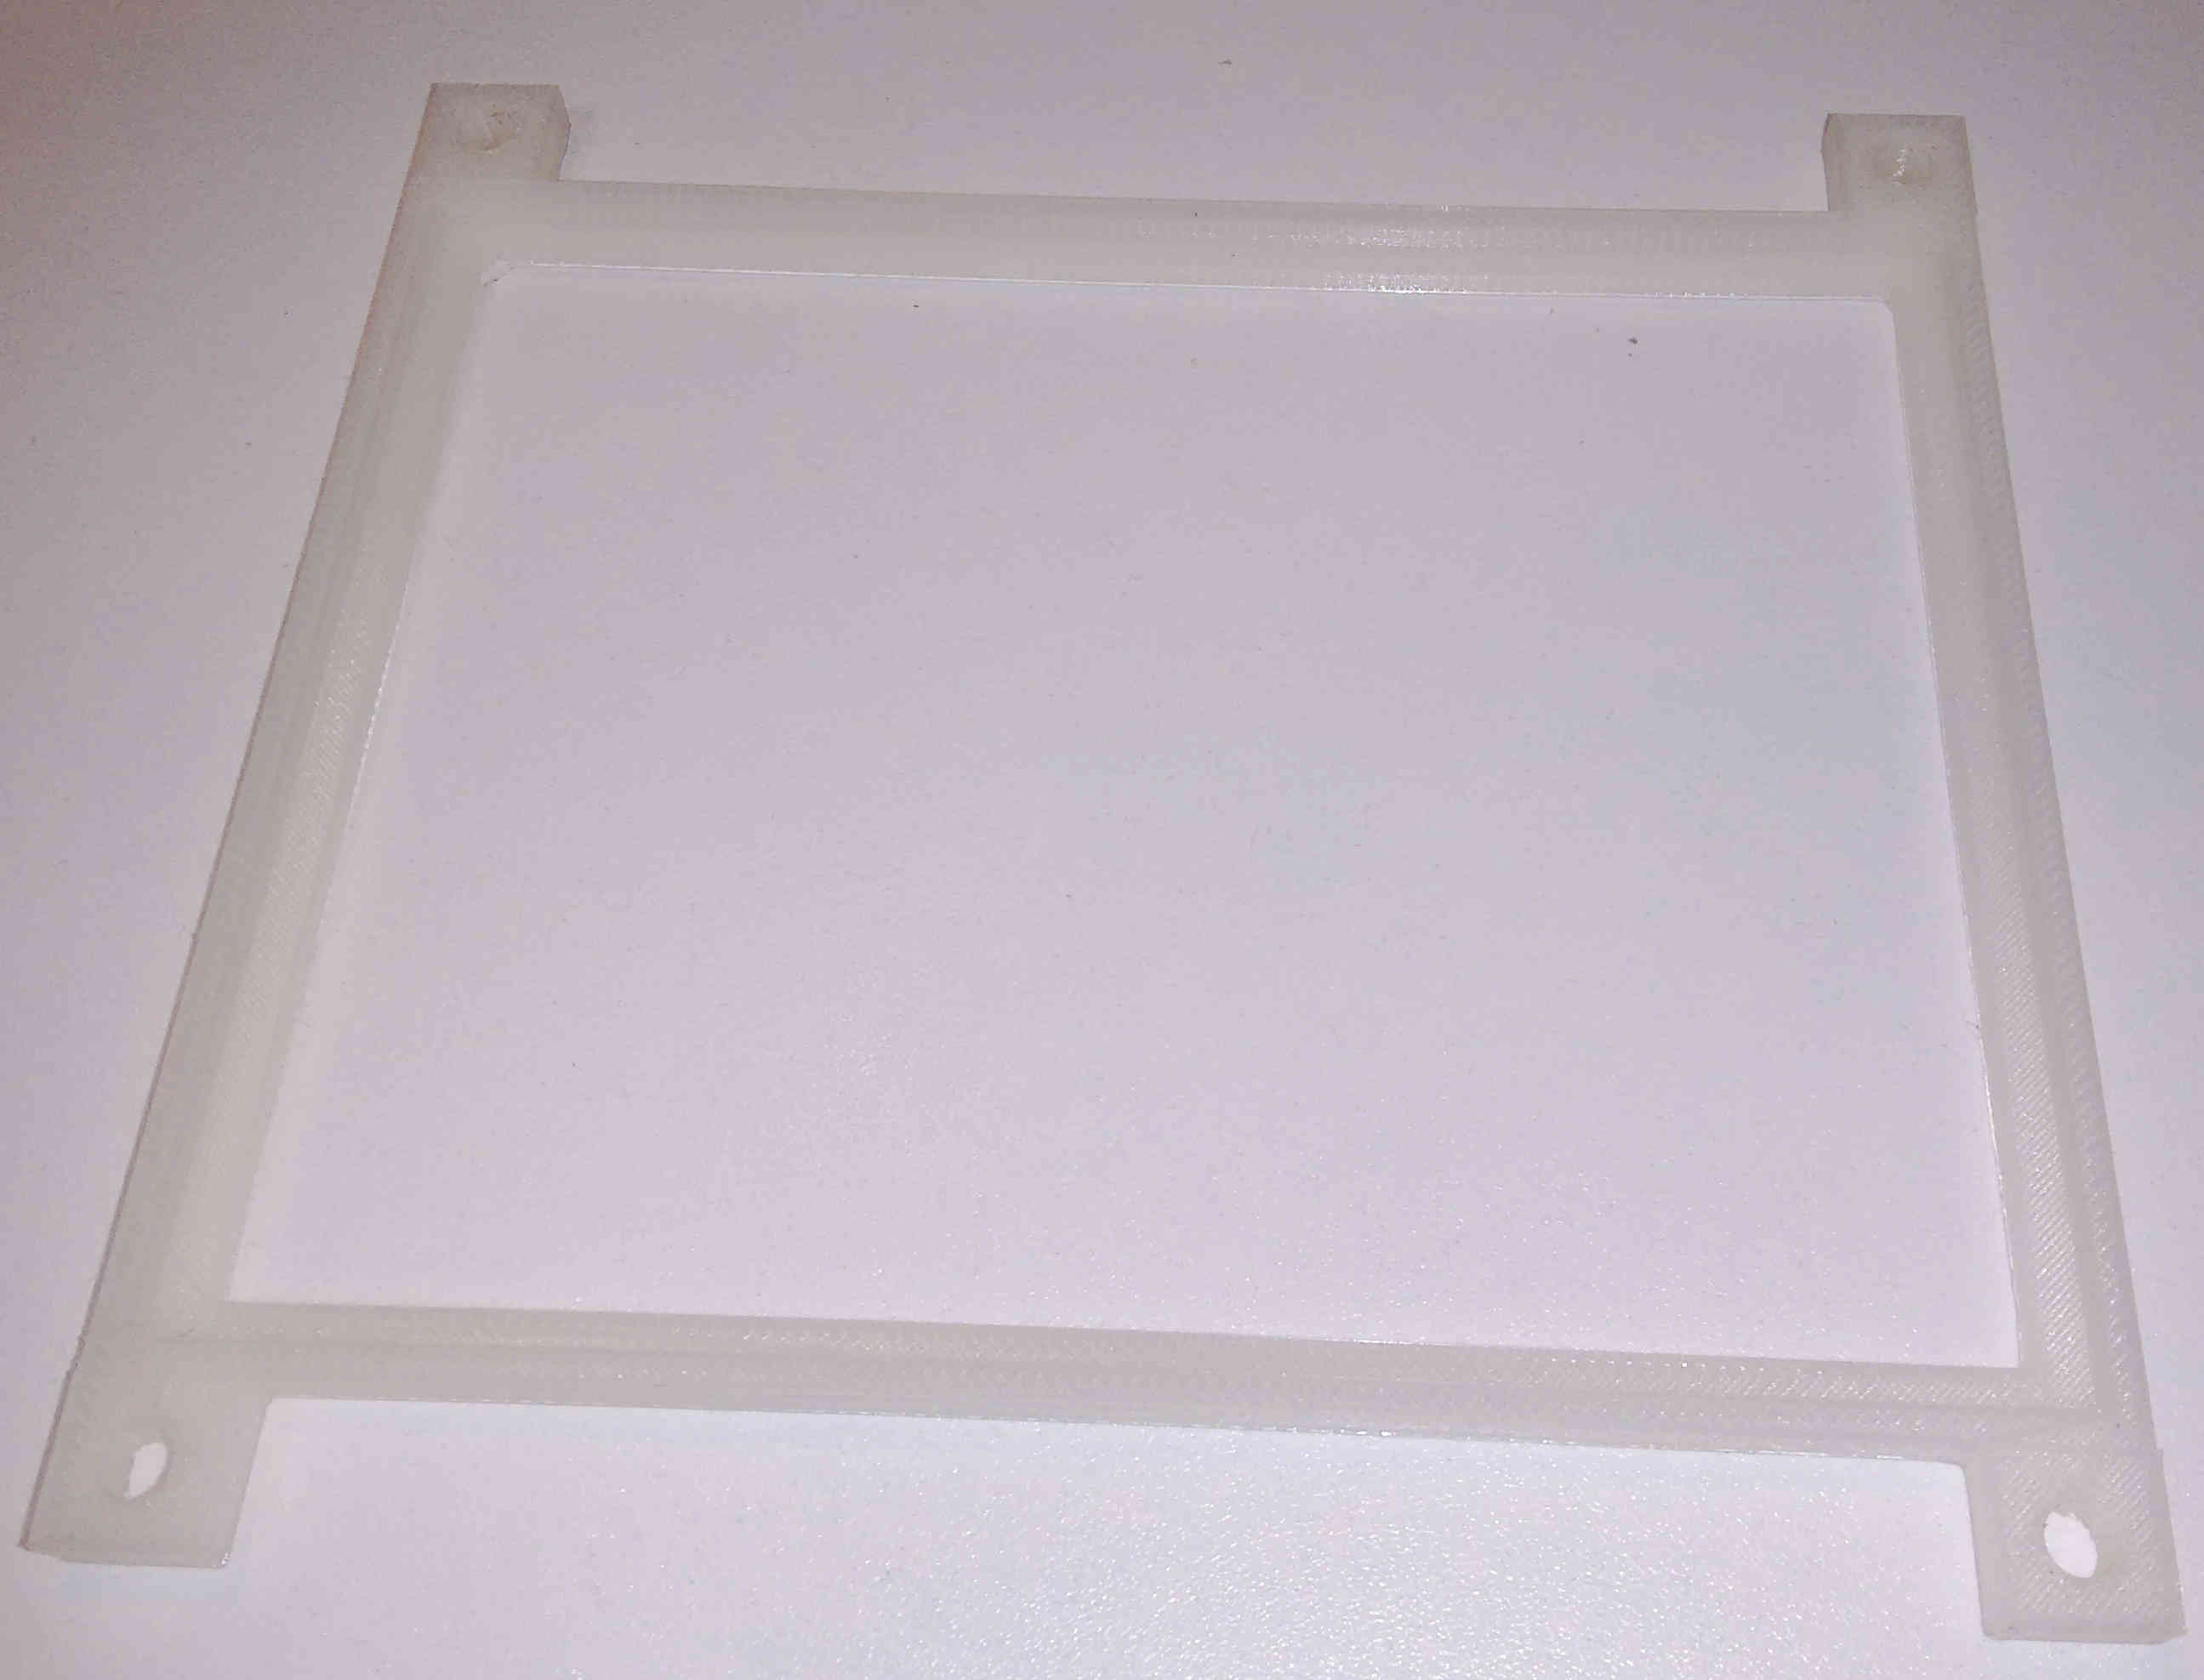
\includegraphics[width=.5\textwidth]{images/techObj/bilder/rahmen}}


Wie der Deckel wird auch der Rahmen massiv gedruckt. Auch hier ist das Ziel, eine hohe Stabilit�t zu erreichen. Dieses Ziel zu erreichen ist beim Rahmen noch wichtiger als beim Deckel, da die Rahmen das gesamte Aufbewahrungssystem zusammenhalten sollen.

Als Infill-Pattern wurde beim Rahmen, ebenso wie beim Deckel, ein konzentrisches Muster gew�hlt. Aufgrund der rechteckigen Form des Rahmens kann der Druckkopf ihn leicht mit einem konzentrischen Muster abfahren.
Abbildung \ref{figure:techObj:druck:rahmen} zeigt den gedruckten Rahmen.


\subsection{Bodenplatte}
\piccaption{Gedruckte Bodenplatte \label{figure:techObj:druck:bodenplatte}}
\parpic[r]{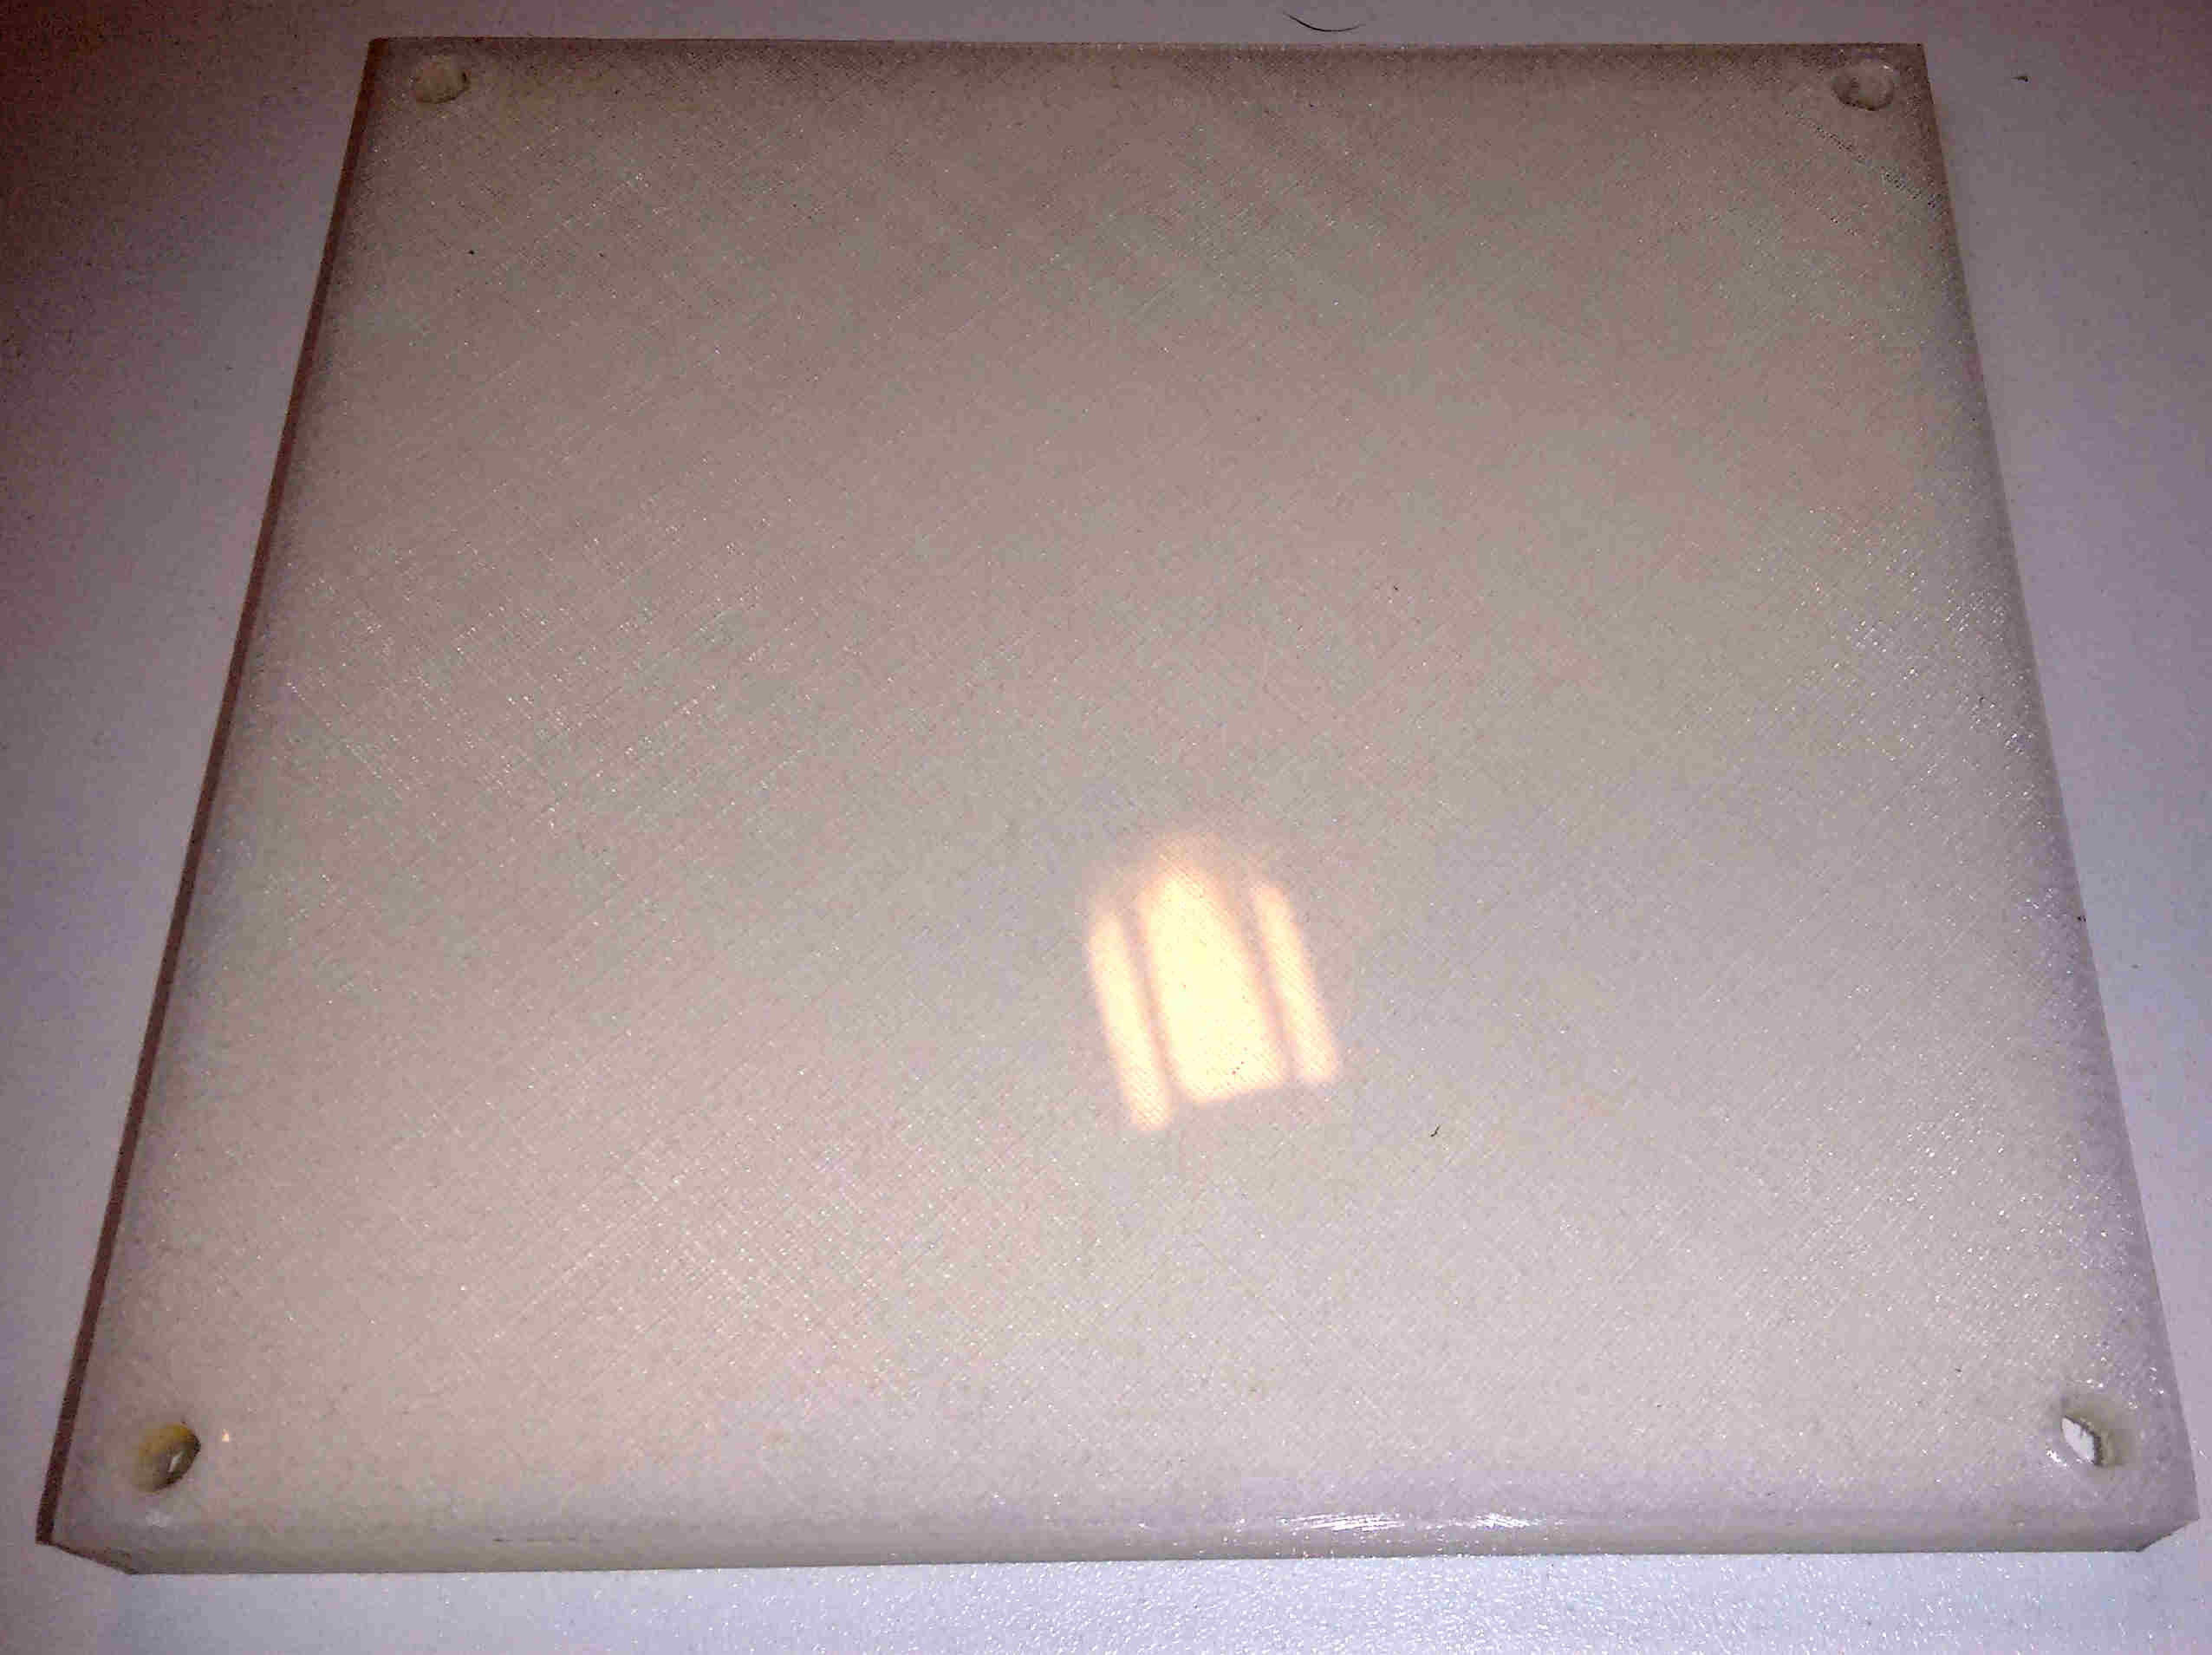
\includegraphics[width=.5\textwidth]{images/techObj/bilder/bodenplatte}}

Zwar ist auch bei der Bodenplatte die Stabilit�t wichtig, aber dadurch, dass sie insgesamt dicker ist als Rahmen oder Deckel, muss sie nicht massiv gedruckt werden. Bei der Bodenplatte wird auch mit 70\% F�llung eine ausreichend hohe Stabilit�t bei einer noch akzeptablen Druckdauer erreicht.
Die gedruckte Bodenplatte ist in Abbildung \ref{figure:techObj:druck:bodenplatte} zu sehen.
Im Gegensatz zu Rahmen und Deckel wird hier kein konzentrisches Infill-Pattern gew�hlt. Stattdessen wird die Bodenplatte mit Linien gef�llt. 


\subsection{Boxen}
Durch die Gr��e der Boxen w�rde ein massiver Druck unverh�ltnism��ig viel Zeit in Anspruch nehmen. Die gew�nschte Stabilit�t kann auch mit nicht ganz ausgef�llten Objekten erzielt werden. Die endg�ltigen Versionen der Boxen f�r den Raspberry Pi und den \ac{USB}-Hub sind zu 90\% gef�llt, f�r die Festplattenbox werden 80\% gew�hlt.

Die Boxen f�r den \ac{USB}-Hub (dargestellt in Abbildung \ref{figure:techObj:druck:boxen:Hub}) und die Festplatte (dargestellt in Abbildung \ref{figure:techObj:druck:boxen:FP}) werden mit konzentrischen Mustern gedruckt. F�r die in Abbildung \ref{figure:techObj:druck:boxen:Pi} abgebildete Raspberry Pi-Box werden Linien verwendet, da der innere Aufbau dieser Box so kompliziert ist, dass er mit konzentrischen Mustern nur schwer auszuf�llen w�re.
 
	\begin{figure}[h!]
		
		
		\begin{minipage}[b]{.305\textwidth}
			
			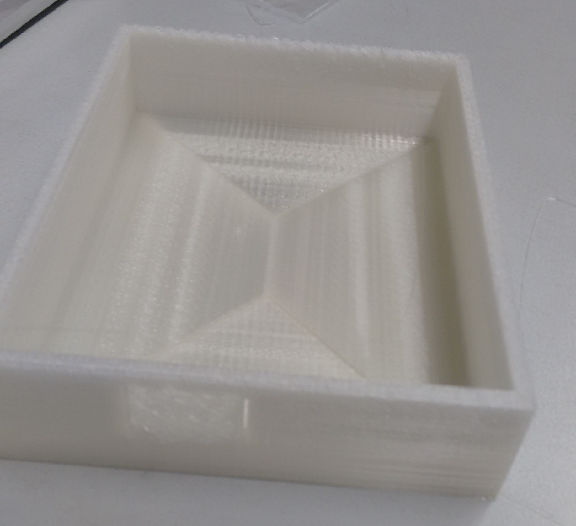
\includegraphics[width=\textwidth]{images/techObj/bilder/FP_Box}
			\subcaption{Festplattenbox}
			\label{figure:techObj:druck:boxen:FP}
			
		\end{minipage}
		\begin{minipage}[b]{.265\textwidth}
			
			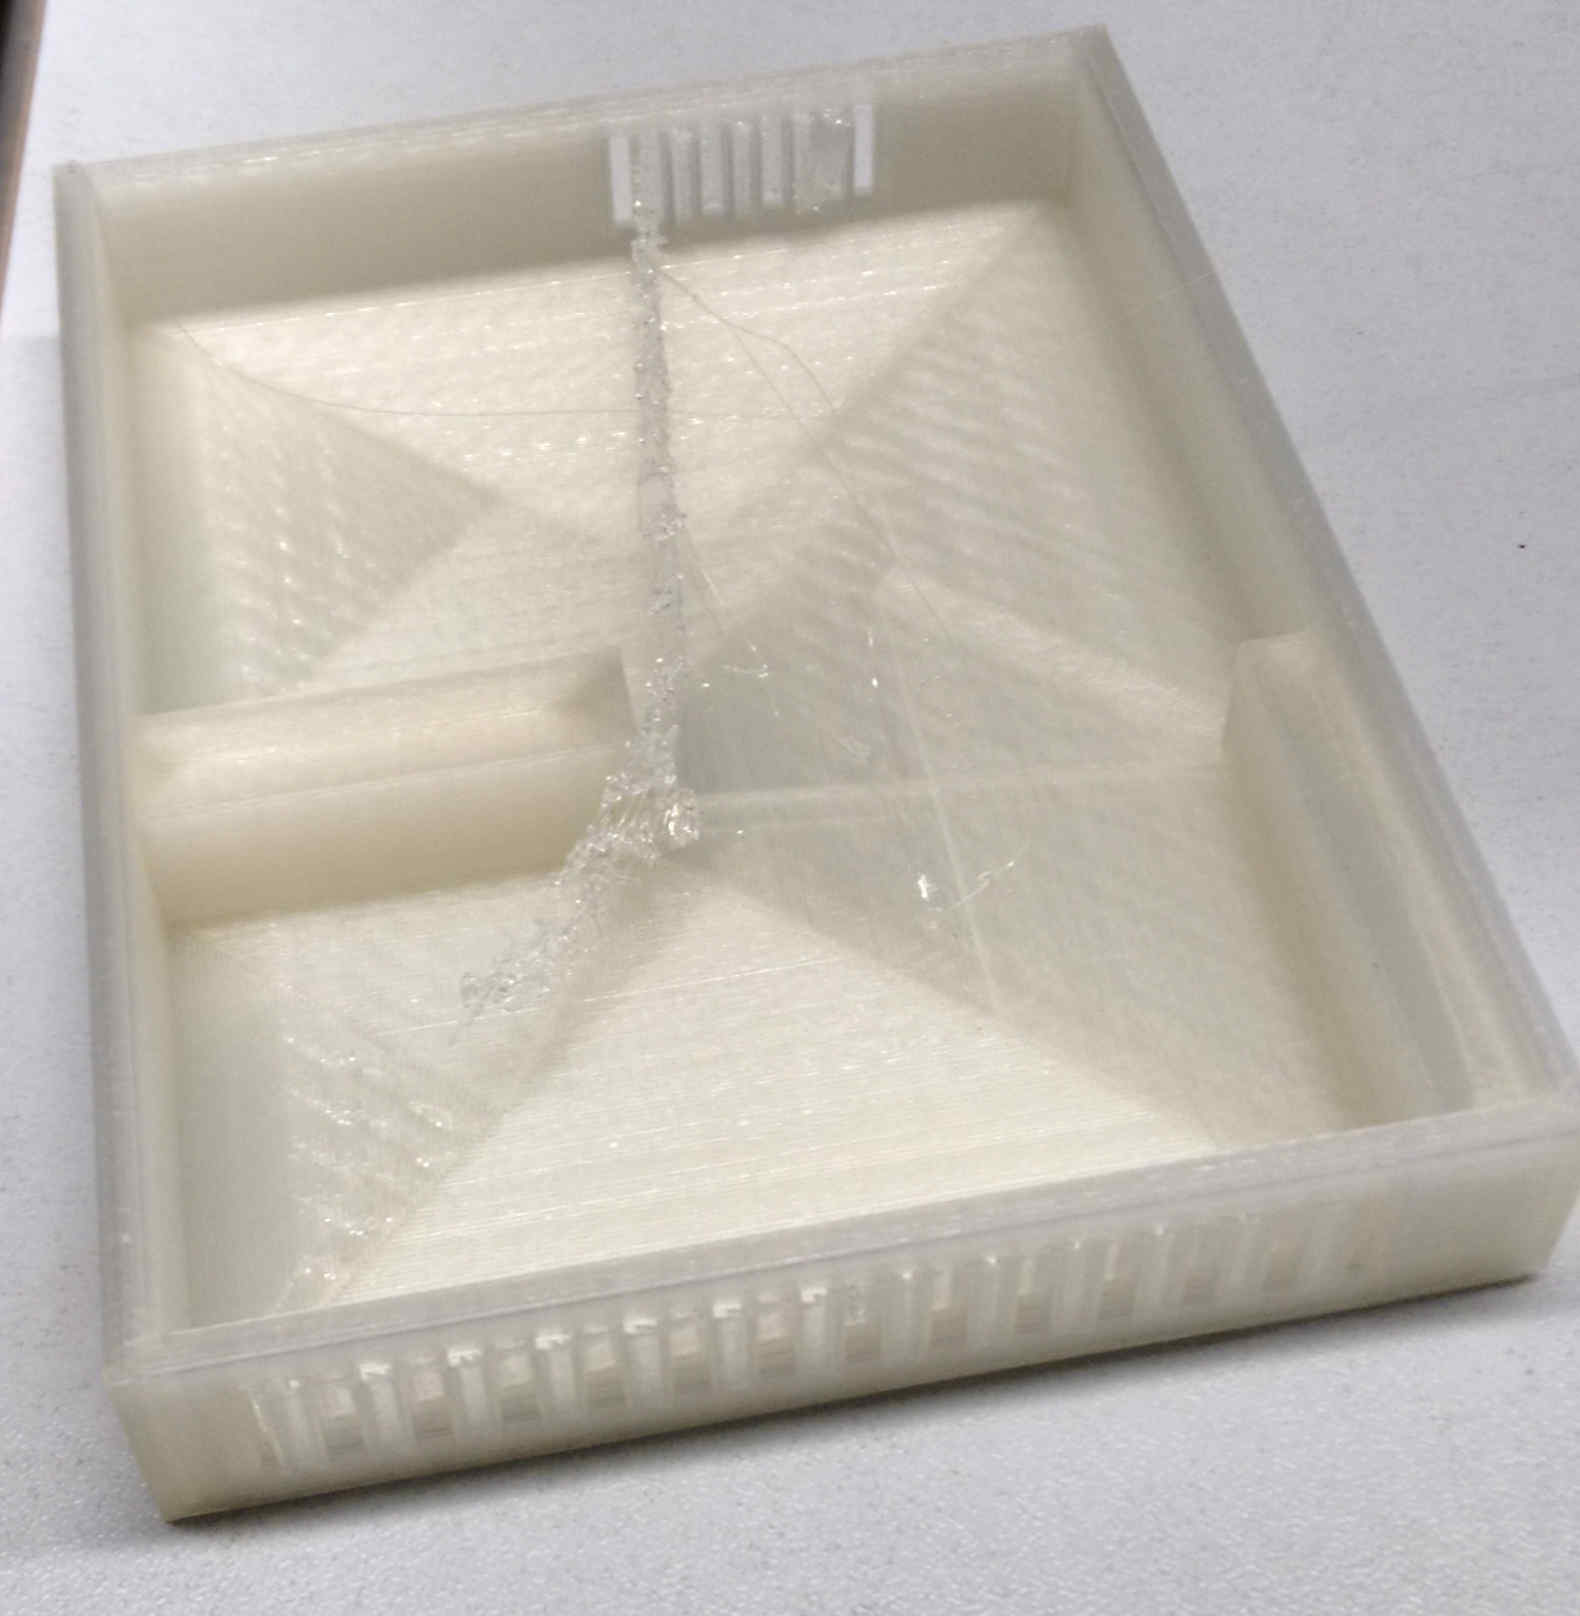
\includegraphics[width=\textwidth]{images/techObj/bilder/Hub.jpg}
			\subcaption{Hub-Box}
			\label{figure:techObj:druck:boxen:Hub}
			
		\end{minipage}
		\begin{minipage}[b]{.34\textwidth}
			
			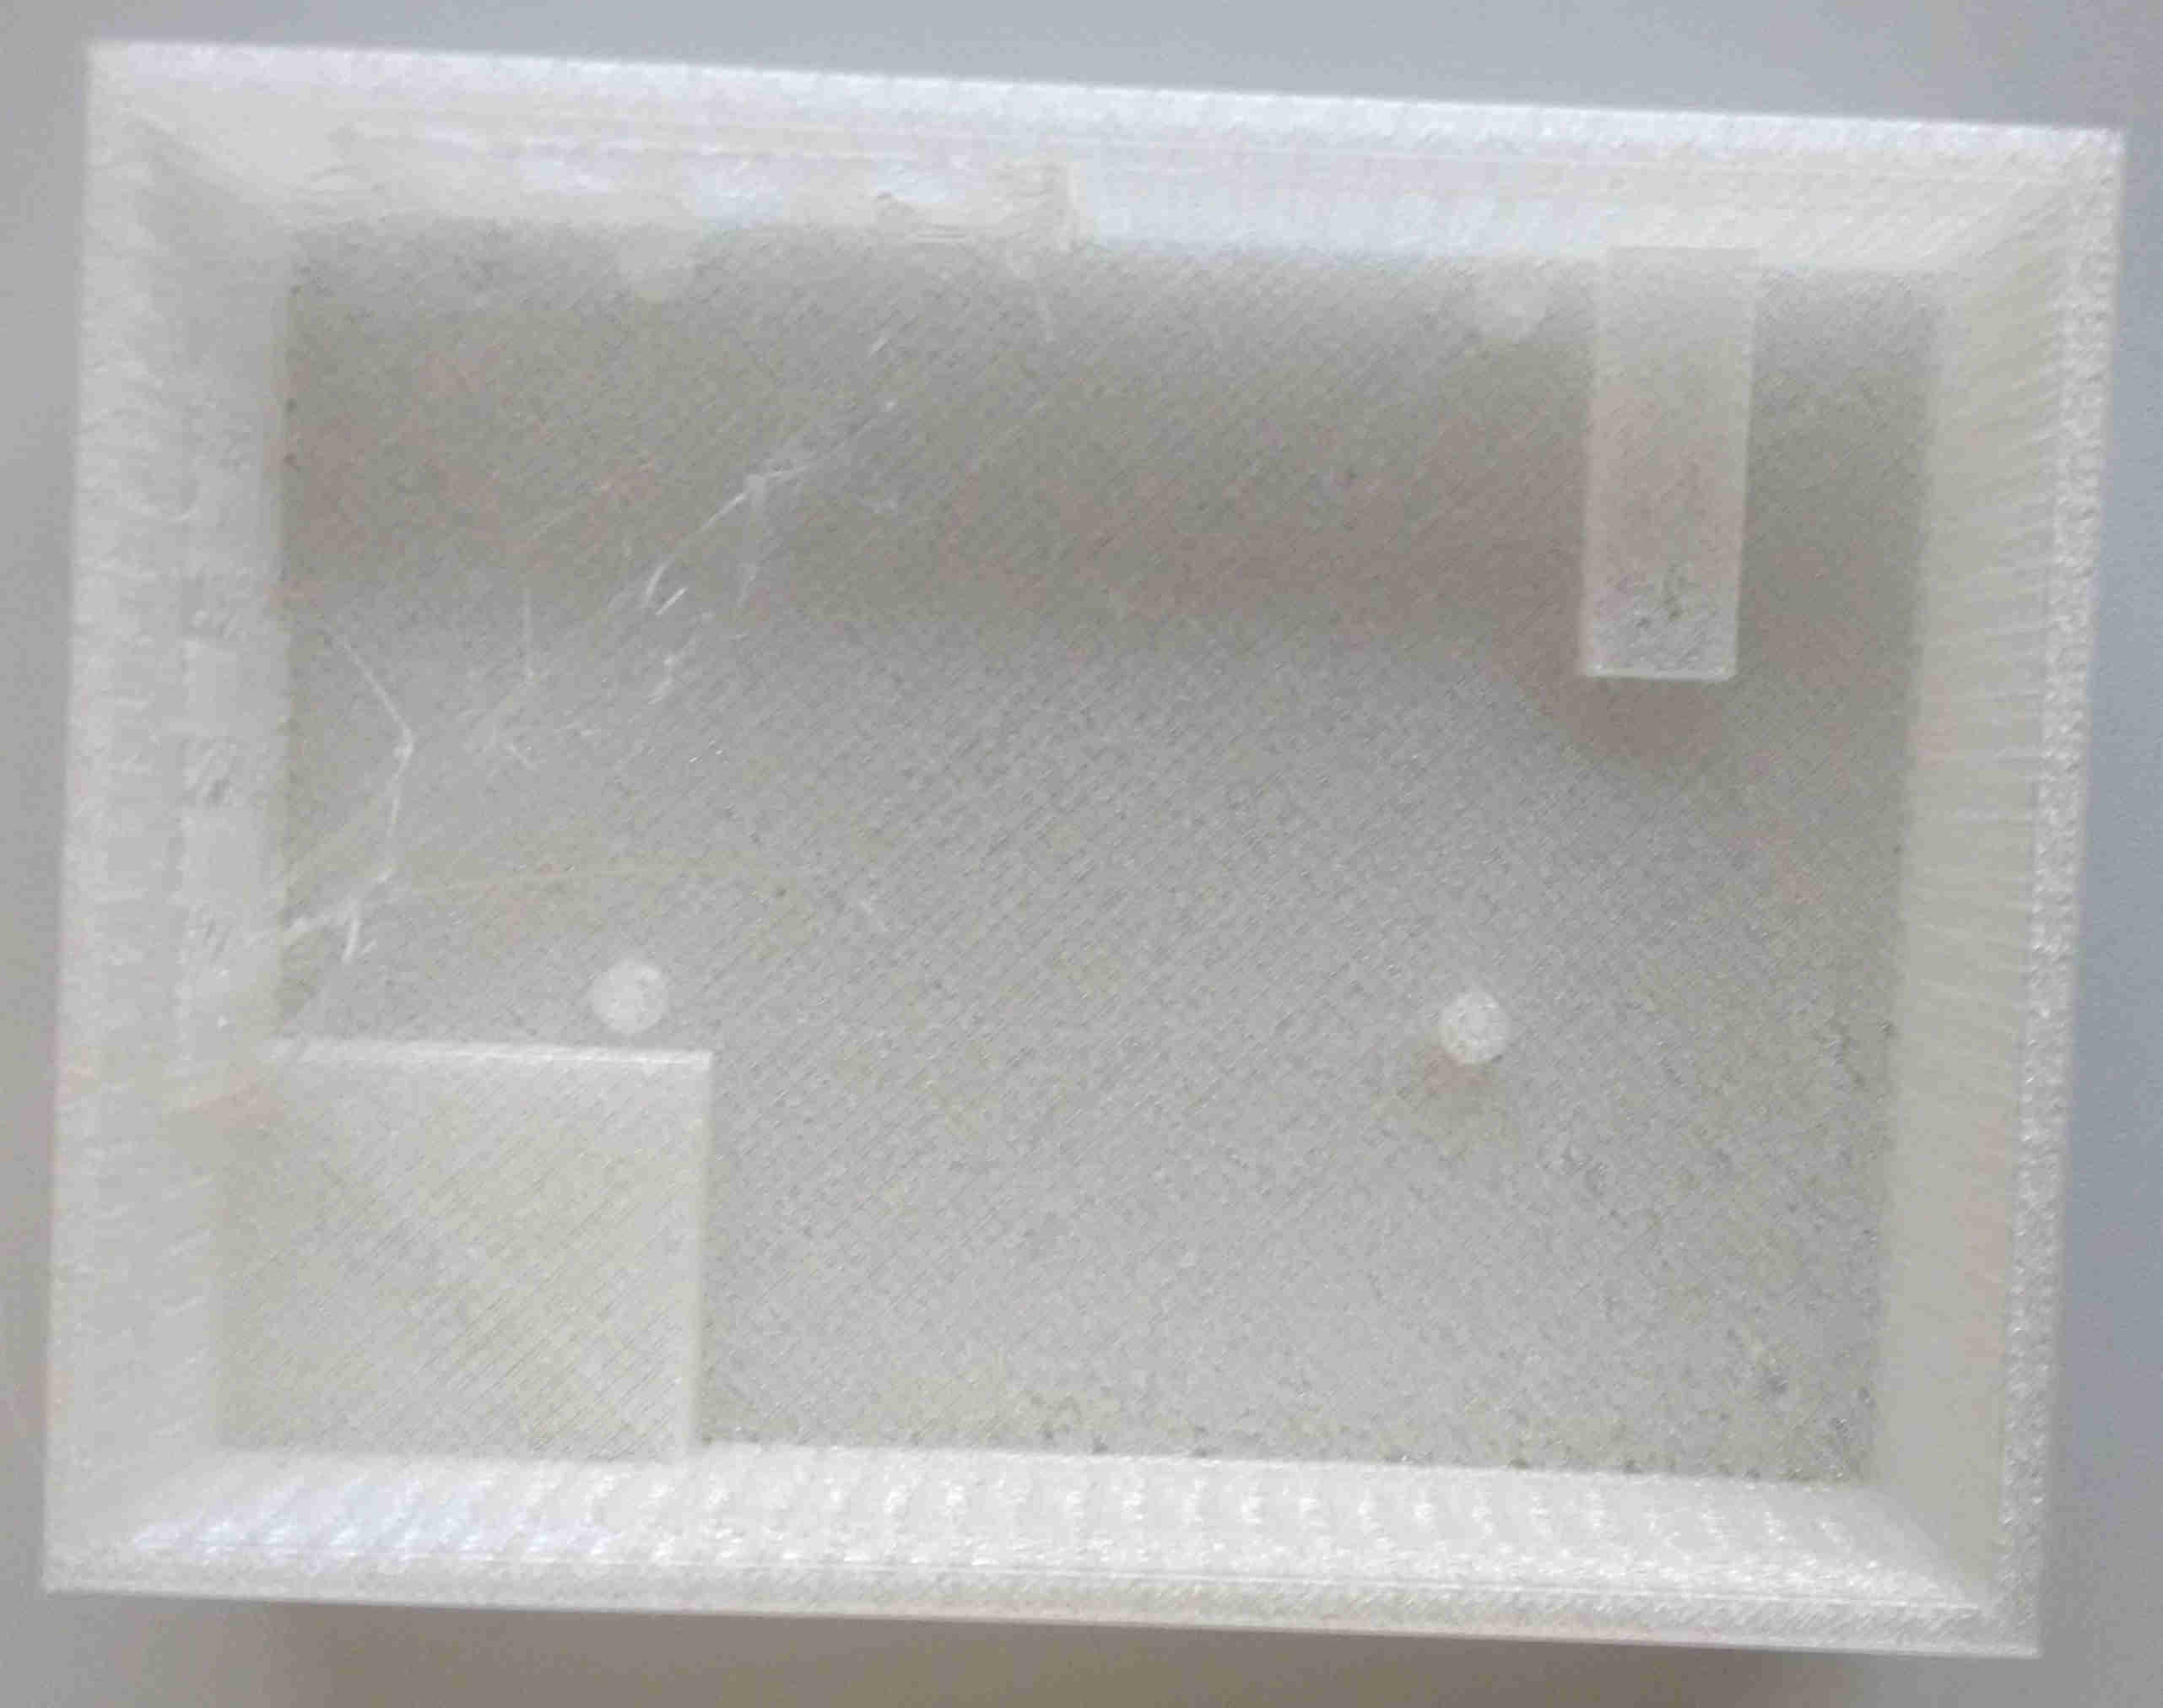
\includegraphics[width=\textwidth]{images/techObj/bilder/PiBox2.jpg}
			\subcaption{Pi-Box}
			\label{figure:techObj:druck:boxen:Pi}
			
		\end{minipage}
		\caption{Gedruckte Boxen}
	\end{figure}




\section{Fazit: Eignung f�r technische Objekte}
% bezogen auf Ultimaker
\piccaption{Zusammengesetztes Aufbewahrungssystem \label{figure:techObj:druck:gesamt}}
\parpic[r]{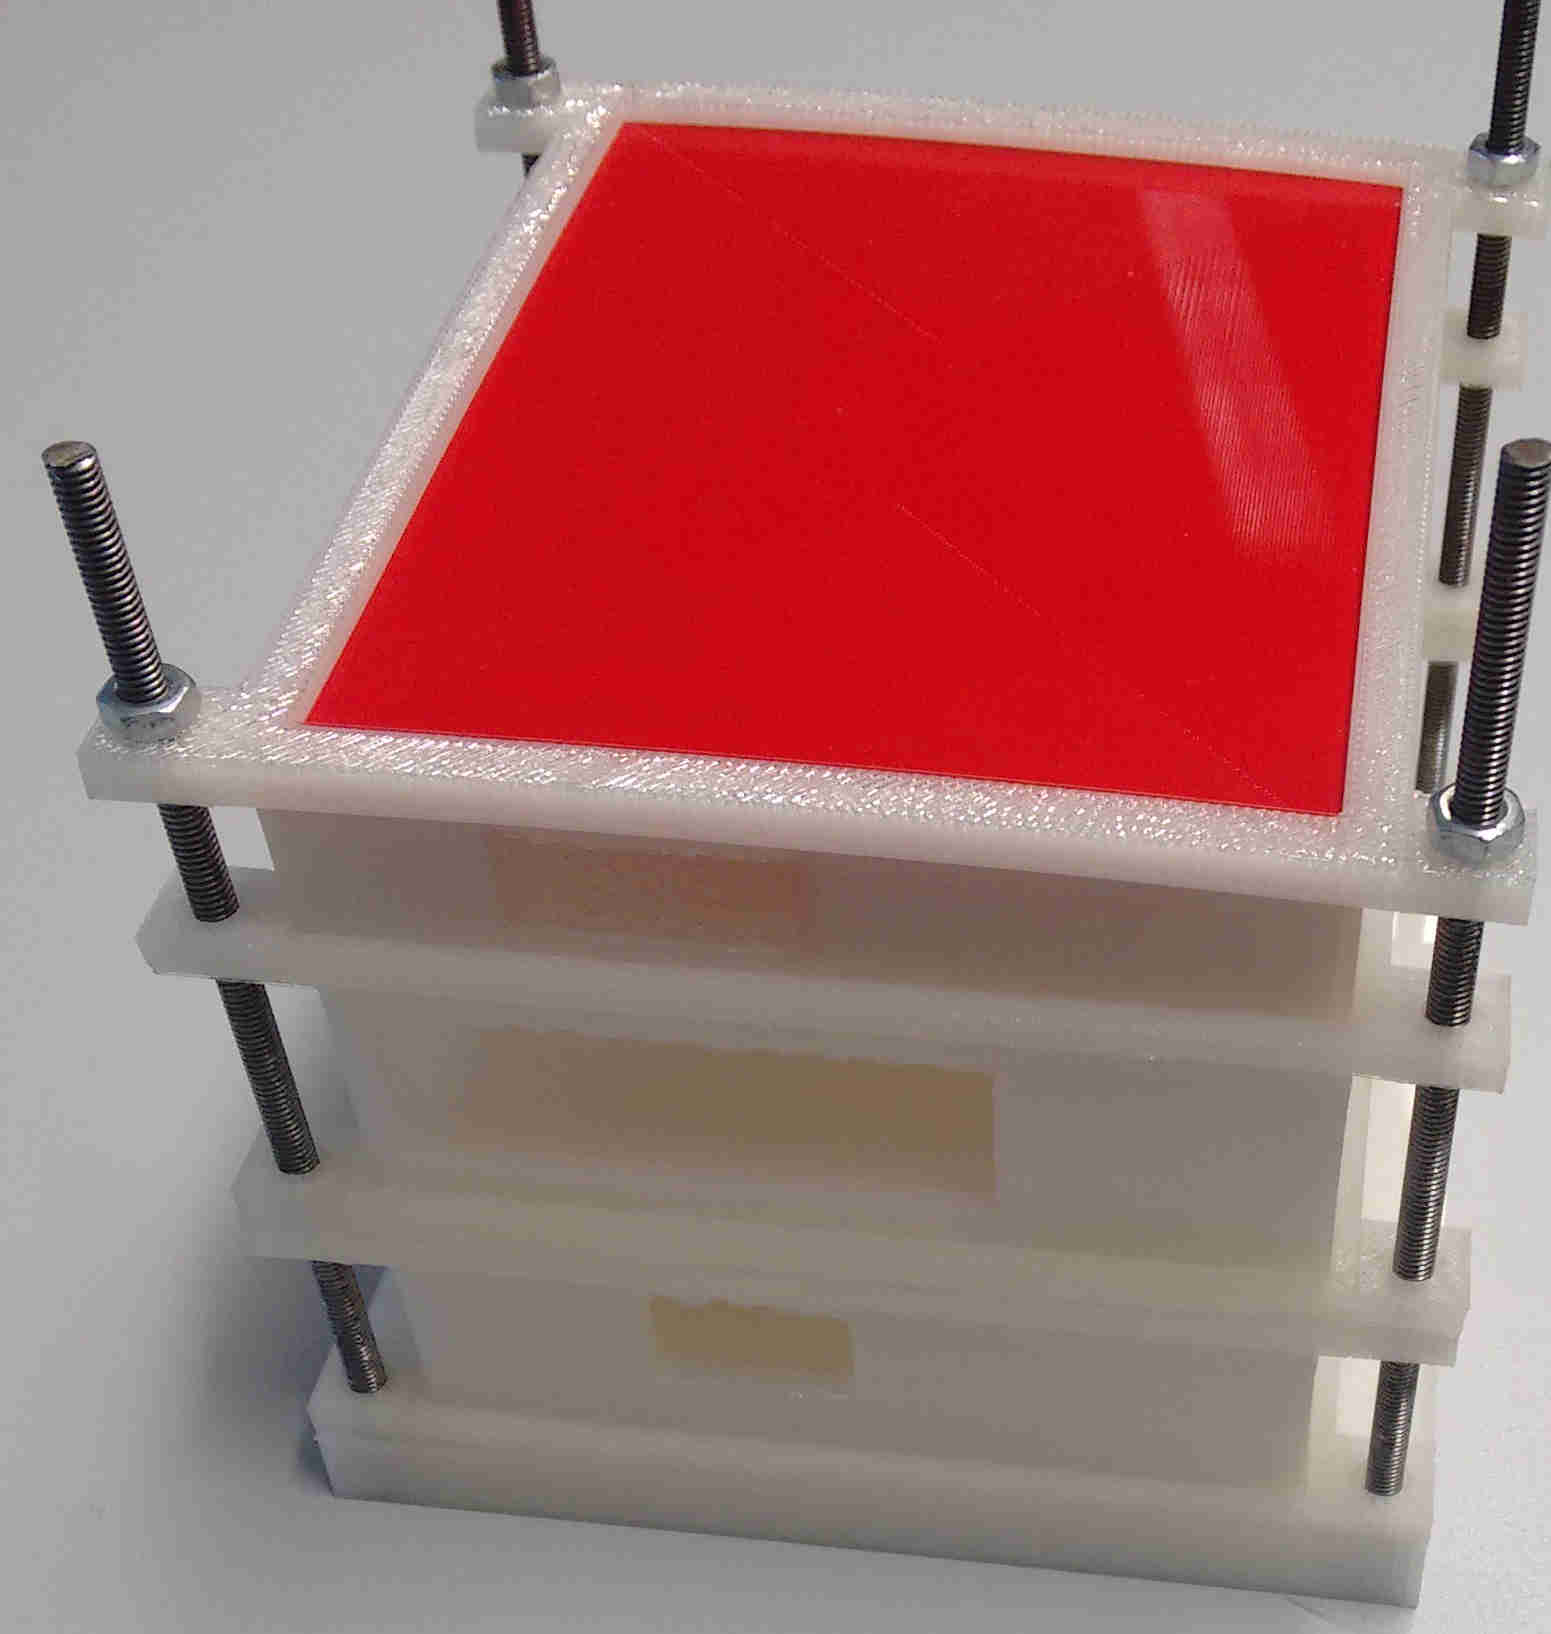
\includegraphics[width=.4\textwidth]{images/techObj/bilder/gesamt_oben}}

Abbildung \ref{figure:techObj:druck:gesamt} zeigt das zusammengesetzte Aufbewahrungssystem. 

Wie bereits eingangs erw�hnt wurde, wurde f�r diese Studienarbeit der Ulitmaker 2 verwendet. Deshalb wird in diesem Fazit auch nur betrachtet, inwiefern sich speziell dieser Drucker eignet, um technische Objekte zu erstellen.

\picskip{0}
\vspace*{8em}

\subsection{Material}
Als Filament f�r den Druck wurde \ac{PLA} verwendet. Bei den Drucken fiel auf, dass die Materialeigenschaften, abh�ngig von der verwendeten Farbe, teilweise deutlich unterschiedlich waren. Am besten gelangen die Drucke mit rotem Filament. Schwarzes Filament dagegen war sehr spr�de. Bei durchsichtigem Filament hielten die verschiedenen Linien teilweise nicht so stark zusammen wie beispielsweise bei rotem Filament, was insbesondere bei konzentrischen Mustern zu einer Instabilit�t f�hrte. Dieses Problem wird in Kapitel \ref{chapter:fehler:material} genauer beschrieben.

Allgemein sollte man beim Ultimaker 2 also vor dem Druck eines gr��eren Objekts testen, welche Farbe die besten Eigenschaften aufweist.


\subsection{Unzureichende Druckgenauigkeit}
Beim Druck des technischen Objekts war auffallend, dass die in Solid Edge definierten und in Cura noch korrekt dargestellten Ma�e der Objekte vom Drucker nicht ma�getreu gefertigt wurden. Dies war besonders auffallend bei einem 1cm x 1cm x 1mm - Quader, den wir zum Testen der aktuellen H�hen-Kalibrierung verwendeten. Die Seitenma�e des Quaders ma�en anstatt einem Zentimeter nur ca. 8 Millimeter. Bei einer Linienbreite von 0.4mm sind das etwa 4 Linien, die vom Slicer nicht zum Drucken vorgesehen wurden. 

Dieses Problem wiederholte sich bei schmalen Strukturen: alle W�nde, die nicht �ber 0.8mm ma�en - also eine beidseitige Wand - wurden von Cura ohne Benachrichtigung beseitigt. Mittels Repetierhost kann das Fehlen der W�nde aufgezeigt werden. In mancher Situation erzeugte Cura auch W�nde, die nicht sein sollten und f�llte trotz deaktivierter Funktion klar definierte Hohlr�ume massiv aus.

Die relativ hohe Ungenauigkeit der Drucke f�hrte teilweise zu Problemen mit den Spaltma�en. Da oft erhebliche Unterschiede zwischen den definierten Ma�en und den Ma�en des gedruckten Objekts bestanden, konnten Objekte nicht passend zusammengesetzt werden. 

Beispielsweise mussten die Deckel f�r die Boxen sowie die Serverh�lle des Raspberry Pi mit angepassten Ma�en erneut gedruckt werden. Manche Objekte mussten zwar nicht erneut gedruckt, aber nachbearbeitet werden, um miteinander kombinierbar zu sein.

Zu dem Zeitpunkt, zu dem das technische Objekt gedruckt wurde, stand nur eine D�se der Gr��e 0.4mm zur Verf�gung. Dadurch war die minimale Breite einer Linie festgelegt. Da f�r das Aufbewahrungssystems keine Strukturen, die feiner als 0.4mm sind, gedruckt werden mussten, stellte dies in unserem Fall kein Problem dar. Allerdings w�re f�r das Drucken von technischen Objekten allgemein eine M�glichkeit, einfach verschieden gro�e D�sen in den Ultimaker 2 einsetzen zu k�nnen, w�nschenswert. Diese Funktion wird durch den Olsson-Block, mit dem der Ultimaker 2 erweitert werden kann, realisiert.

F�r das Aufbewahrungssystem war die Genauigkeit des Ultimaker 2 ausreichend, auch wenn einige Objekte erneut mit h�heren Toleranzen gedruckt werden mussten. Da technische Objekte im Allgemeinen jedoch mit minimalen Abweichungen angefertigt werden sollten, sind die Abweichungen des Ultimaker 2 an sich zu hoch. Sie zeigen, dass der Ultimaker 2 nicht die notwendige Pr�zision liefern kann, die f�r technische Objekte in der Regel erforderlich ist.





	\chapter{Entwicklung eines organischen Objekts}
		%	% TODO: Label auf technisches Objekt
	
	\chapter{Entwicklung eines organischen Objekts} 
	\label{chapter:orgObj}
%	%TODO Einleitung: Idee
	% explizite Bezug auf Ultimaker 2, andere Drucker liefern andere Ergebnisse
	% Besonderheiten eines organischen Objekts

	Das Ziel dieser Studienarbeit ist es, zwei unterschiedliche Objekte zu designen und zu drucken. Im vorherigen Kapitel \ref{chapter:techObj} wird die Entwicklung eines technischen Objekts beschrieben. Bei einem technischen Objekt sind die Anspr�che an genaue Bema�ungen hoch, das Objekt selbst sollte so einfach wie m�glich gestaltet sein. Dadurch besteht es oft aus einfachen geometrischen Formen. Allgemein liegt der Fokus auf der Funktionalit�t des Objekts. Um technische Objekte zu designen, wird in der Regel eine \ac{CAD}-Software verwendet. \\
	In diesem Kapitel wird eine andere Art eines Objekts beschrieben: Das organische Objekt. Im Gegensatz zu einem technischen Objekt steht hier nicht die reine Funktionalit�t im Vordergrund. Organische Objekte sind Objekte, die in der Natur vorkommen und nicht k�nstlich vom Menschen gefertigt wurden, beispielsweise Lebewesen oder Pflanzen. In der Regel besitzen diese Objekte kaum Ecken, Kanten oder gerade Fl�chen. 
	
	Im Folgenden werden das Design und der Druck eines solchen Objekts beschrieben, im Anschluss folgt ein Fazit �ber die generelle Eignung des Ultimaker 2 f�r den Druck organischer Objekte.
	Wie bereits im vorigen Kapitel bezieht sich diese Arbeit auf den Ultimaker 2, der im Kapitel \ref{chapter:techGr:ultimaker2} vorgestellt wird. In der Arbeit mit einem anderen Drucker k�nnen sich Vorgehensweise und Ergebnis deutlich unterscheiden.
	

	\section{Konzept}
	\label{chapter:orgObj:konzept}
% --> "Strichm�nnchen"
	Wie zu Beginn des Kapitels beschrieben, soll das organische Objekt runde, gew�lbte Fl�chen besitzen. F�r diese Studienarbeit wurde ein dreidimensionales Strichm�nnchen als Objekt gew�hlt. Dieses kann unter Verwendung mehrerer Zylinder und Kugeln modelliert werden und enth�lt somit einige gew�lbte Fl�chen. 
	Der Kopf des Strichm�nnchens wird als Kugel modelliert, der restliche K�rper besteht aus sieben Zylindern. Einer davon dient als K�rper und je ein Zylinder wird verwendet, um ein Bein zu modellieren. Die Arme werden mit je zwei Zylindern modelliert. Dadurch kann ein Ellbogengelenk simuliert werden und abwechslungsreiche Armhaltungen werden erm�glicht.  
	
	
	
%	%TODO ist eigenes Kapitel Entwurf n�tig?
	\section{Entwurf}
	% Arbeit mit Blender
	
	\piccaption{Design des organischen Objekts  \label{fig:orgObj:orgObj}}
	\parpic[r]{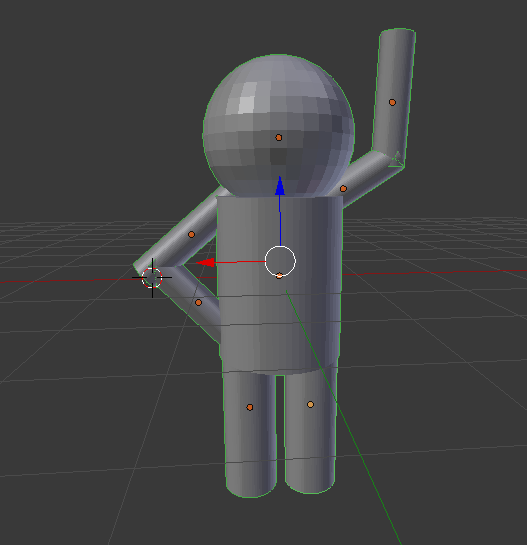
\includegraphics[width=.3\textwidth]{images/orgObj/orgObj}}
	
	
	Das im vorigen Abschnitt beschriebene dreidimensionale Strichm�nnchen wird mithilfe der Software Blender (Kapitel \ref{chapter:sdt:blender}) modelliert. Es wird modelliert, indem verschiedene geometrische Grundk�rper zusammengesetzt werden.
	
	Wie im vorigen Abschnitt \ref{chapter:orgObj:konzept} beschrieben, wird das M�nnchen aus sieben Zylindern und einer Kugel zusammengesetzt. Abbildung \ref{fig:orgObj:orgObj} zeigt einen Screenshot des modellierten M�nnchens in Blender.
	
	Sowohl Zylinder als auch Kugeln werden in Blender als Grundk�rper zur Verf�gung gestellt. Die Bema�ung der Objekte kann jeweils angepasst werden. Diese K�rper werden in den Viewport gezogen und verschoben, bis sie sich an der gew�nschten Position befinden. Beim Verschieben ist es m�glich, den K�rper nur entlang einer Gerade (eindimensional) oder in einer Ebene (zweidimensional) zu verschieben.
	
	Wenn sich alle Grundk�rper an der gew�nschten Position befinden, markiert man sie und f�gt sie zu einer Gruppe zusammen. Diese Gruppe kann dann als \ac{STL}-Datei gespeichert werden. 



%	\newpage
	
	\section{Druck des Objekts}
	% Wie w�re es ideal gewesen?, fertiges Objekt 
	% Welche Parameter? --> spezifisch beim organischen Objekt
	% Verlinkung zu Fehlern

	
	Im Gegensatz zum technischen Objekt (Kapitel \ref{chapter:techObj}), bei dem die Genauigkeit des Drucks sehr wichtig ist, liegt beim organischen Objekt der Fokus darauf, wie gut der Ultimaker 2 gew�lbte Fl�chen drucken kann.
	
	
	Zu Testzwecken wird das Objekt in zwei verschiedenen Positionen gedruckt. Einmal wird das M�nnchen liegend auf der Druckplatte positioniert, einmal stehend. Dadurch kann untersucht werden, ob es einen Unterschied macht, wie das Objekt platziert wird. 
	
	Das liegende M�nnchen hat insgesamt mehr Auflagefl�che als das stehende M�nnchen, wodurch es allerdings auch durch mehr Supportstrukturen gest�tzt werden muss. Daf�r muss nicht weit nach oben gedruckt werden und es m�ssen keine �berh�nge gedruckt werden.\\
	
	Das stehende M�nnchen hat insgesamt weniger Kontakt mit der Druckplatte, ben�tigt aber dennoch kaum Supportstrukturen, da es mit den unten glatten Beinen auf der Platte steht. Daf�r m�ssen hier f�r die Arme und den Kopf teilweise relativ starke �berh�nge gedruckt werden.
	
	\begin{figure}[h!]
		\begin{minipage}{.5\textwidth}
			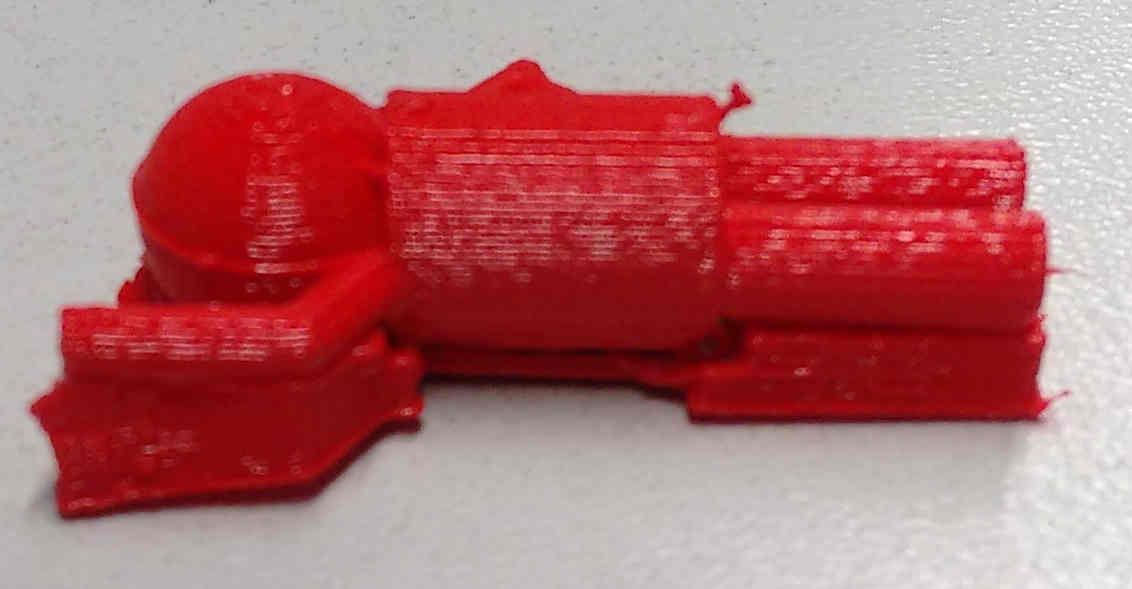
\includegraphics[height=10em]{images/orgObj/oO_liegend}
			\subcaption{Liegende Positionierung}
			\label{fig:orgObj:Druck:liegend}
			%			\subcaption{liegender Druck}
		\end{minipage}
		\begin{minipage}{.5\textwidth}
			\centering
			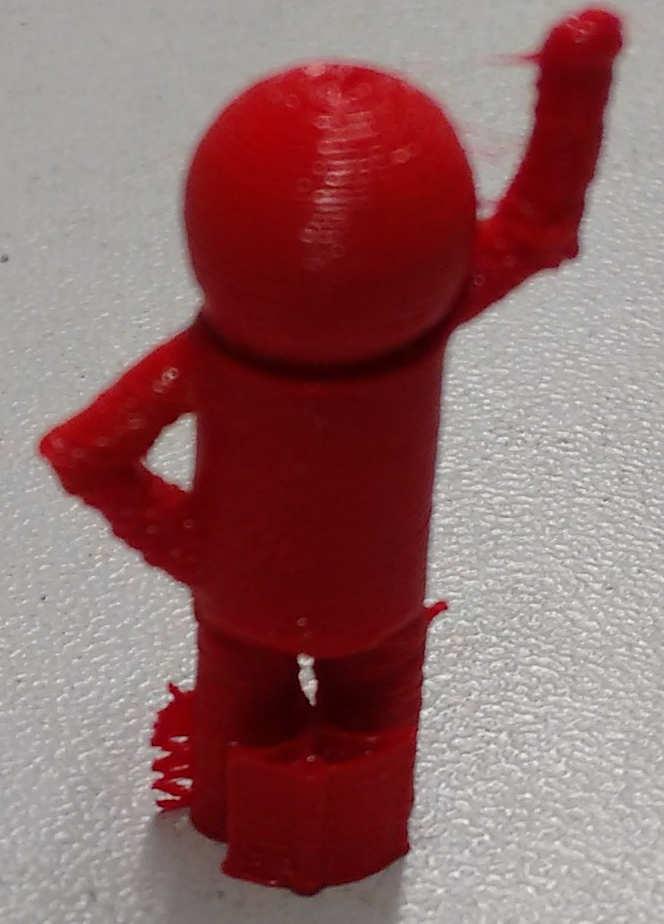
\includegraphics[height=10em]{images/orgObj/oO_stehend}
			\subcaption{Stehende Positionierung}
			\label{fig:orgObj:Druck:stehend}
			%			\subcaption{stehender Druck}
		\end{minipage}
		\caption{Druck des organischen Objekts in verschiedenen Positionierungen}
		\label{fig:orgObj:Druck}
	\end{figure}
		
	
	Abbildung \ref{fig:orgObj:Druck} zeigt die beiden mit verschiedenen Positionierungen gedruckten M�nnchen.
	
	Die �berh�nge des stehenden M�nnchens sind gut gelungen, sogar ohne durch Supportstrukturen abgest�tzt zu werden. Die vergleichsweise geringe Auflagefl�che auf der Druckplatte stellt kein Problem dar, da die F��e einen guten Halt bieten. Auch die Kugel, die den Kopf des M�nnchens darstellt, ist gut und rund geworden. 
	
	Beim liegenden M�nnchen dagegen sind viele Supportstrukturen n�tig, damit es gen�gend Auflagefl�che auf der Druckplatte besitzt. Diese Strukturen lassen sich nur schwer und nicht r�ckstandslos vom Objekt l�sen. Auff�llig ist zudem, dass die Kugel, die den Kopf darstellt, eine starke Kante in der Mitte aufweist. 
	
	Allgemein ist das stehende M�nnchen deutlich besser gelungen als das liegende. 
	
	
%	\piccaption{Druck des stehenden organischen Objekts  \label{fig:orgObj:oO_stehend}}
%	\parpic[r]{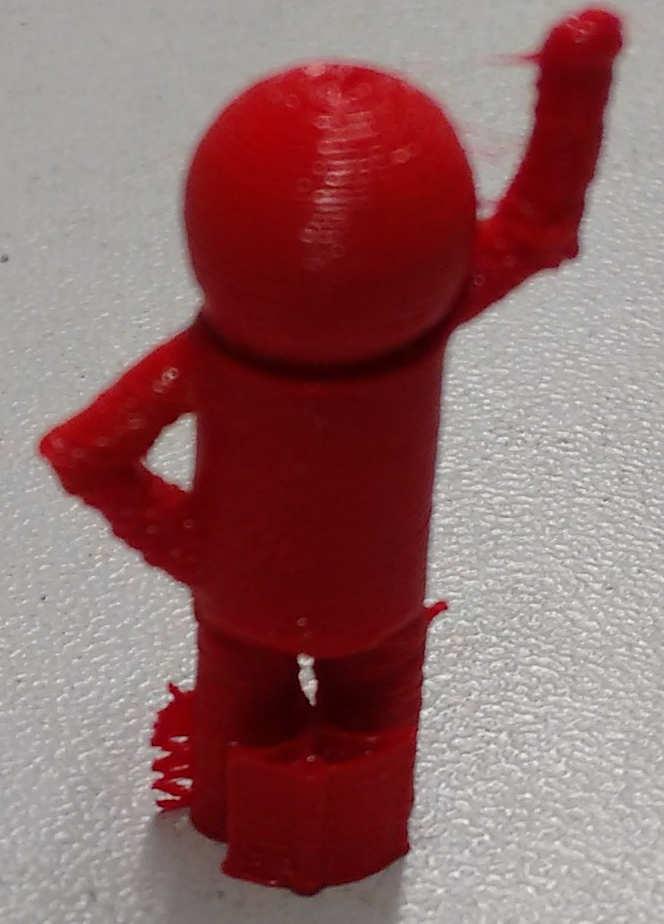
\includegraphics[width=.2\textwidth]{images/orgObj/oO_stehend}}	
%	
%	\picskip{0}
	
	% \section{Aufgetretene Fehler}\frac{Z�hler}{Nenner}
	% Bilder
	% Fehleranalyse, [Ma�nahmen --> technische Grundlagen]
	
	\section{Fazit: Eignung f�r organische Objekte}
	% bezogen auf Ultimaker
	%an sich: kann gut runde Objekt drucken
	%vorsicht bei support strukturen --> m�glichst gro�e auflagefl�che sollte vorhanden sein
	%
	In diesem Kapitel werden das Design und der Druck eines organischen Objekts, also eines Objekts, die viele runde Fl�chen besitzt, beschrieben. Anhand des Drucks eines dreidimensionalen Strichm�nnchens mit dem Ultimaker 2 l�sst sich sagen, dass der Ultimaker 2 prinzipiell geeignet ist, um organische Objekte zu drucken.
	
	Die runden Fl�chen des dreidimensionalen Strichm�nnchens, insbesondere die Kugel, die den Kopf darstellt, sind gut gelungen. Solange sie nicht zu starke �berh�nge aufweisen, kann der Ultimaker runde Fl�chen �berzeugend drucken.
	
	Allerdings sollte das zu druckende Objekt gen�gend gerade Fl�chen besitzen, mit denen es auf der Druckplatte platziert werden kann. Ein Objekt mit einer abgerundeten Fl�che auf der Druckplatte zu platzieren und mit Supportstrukturen abzust�tzen ist nicht empfehlenswert. Wie sich bei dem liegend gedruckten M�nnchen gezeigt hat, lassen sich diese Supportstrukturen kaum r�ckstandslos vom Objekt trennen.
	
	 
	
	
	�oijfdv�idfv�ldfjv	\cite{Hompel2011}.
	
	\chapter{Website}
	
	
	
	\chapter{Zusammenfassung und Ausblick}
	\chapter{Zusammenfassung und Ausblick}
	
	%TODO Diskussion, was davon drinbleibt
	%TODO Organisches Objekt noch nicht erw�hnt
	%TODO Fazit mehr auf unsere Arbeit und weniger auf die Tech beziehen?
	
	Das Ziel der Studienarbeit, n�mlich das Entwerfen und Drucken eines technischen und eines organischen Objekts mit dem Ultimaker 2, wurde erreicht. 
	
	Zus�tzlich zu diesen in Kapiteln \ref{chapter:techObj} und \ref{fig:orgObj:orgObj} beschriebenen Objekten wurden einige kleinere Objekte gedruckt, die in der Regel nicht selbst designt waren. 
	%TODO: Verweise auf Seiten wie Thingiverse? bzw diese Objekte �berhaupt erw�hnen?
	
	
	Ein Gro�teil der Arbeitszeit verlor sich in der Fehlersuche -Vermeidung. Ein gro�er Teil der Drucke scheiterte an sich �hnelnden Fehlern - zu wenig gef�rdertes Material oder zu geringe Haftung am Druckbett. Beides l�sst auf Hardware-/Mechanik-Probleme des Druckers schlie�en.
	
	\section{Technisches Objekt}
	Als technisches Objekt wurde ein Aufbewahrungssystem f�r einen Raspberry Pi, der mit einer Festplatte und einem \ac{USB}-Hub gekoppelt ist, entworfen. Dieses System wurde in Solid Edge mit den korrekten Bema�ungen entworfen. 
	
	Einige der Komponenten des Aufbewahrungssystems wegen Fehldrucken mehrfach gedruckt werden mussten. Zudem mussten die Bema�ungen angepasst werden, da anfangs die Pr�zision des Druckers �bersch�tzt wurde und die Komponenten deshalb nicht ineinander passten. 
	
	Letztlich gelang es jedoch, s�mtliche Komponenten des Aufbewahrungssystems erfolgreich zu drucken. Es wird von einem der Bearbeiter verwendet und stellt eine erhebliche Verbesserung zu dem davor verwendeten Aufbewahrungssystem aus Lochblechen dar.
	
	
	\section{Organisches Objekt}
	Das dreidimensionale Strichm�nnchen, das als organisches Objekt in Blender entworfen wurde, konnte ebenfalls gedruckt werden. W�hrend des Drucks wurden verschiedene Positionen des M�nnchens - liegend und stehend - getestet. 
	
	Dies zeigte, dass Objekte m�glichst eine gerade Auflagefl�che bieten sollen, da die von Cura erstellten Supportstrukturen nur schwer vom Objekt zu l�sen sind.
	
	Das Strichm�nnchen selbst k�nnte noch feiner designt werden, beispielsweise k�nnten Merkmale wie Gesichtsz�ge oder Kleidung hinzugef�gt werden.
	
	% Olsson-Block als Ausblick auf weitere Studienarbeiten
	\section{Upgrade des Druckers}
	Zus�tzlich zu den beschriebenen Objekten wurde der Olsson-Block in den Ultimaker 2 eingebaut. Dieser erm�glicht es zuk�nftig, Drucke mit verschieden gro�en, relativ einfach austauschbaren D�sen zu realisieren. 
	
	Somit k�nnten sich weitere Studienarbeiten mit dem Ultimaker 2 insbesondere auf die Arbeit mit dem Olsson-Block und den neuen M�glichkeiten, die dieser bietet, befassen.

		
%	vermeintlich Design-Problemen des Druckers. Zum Beispiel litt das Werkzeug an notorischer Unterf�rderung des Materials. Zu untersuchen w�re hierbei die Begr�ndung des Drucker-Herstellers das Upgrade des Ultimakters 2 zum 2+ durchzuf�hren. In dem Rahmen wurde der Feeder um ein Getriebe erweitert, das das zum F�rdern n�tige Drehmoment reduziert.
	
	% Der pikierte Unterton sollte noch raus...
	
		
		\section{Fazit zu Additiven Fertigungsverfahren}	
	% Drucktechnologie im privaten Bereich ausgereift?
		F�r den Privatgebrauch lohnt sich ein \ac{3D}-Drucker des heutigen Entwicklungsstands kaum. Die Drucktechnologie ist nicht ausgereift genug, um wartungsarm betrieben zu werden. Die langen Druckzeiten und die n�tigen Vorbereitungen bis zum Druck, ein Objekt zu suchen oder zu designen, die geringen Baugr��en der heutigen kosteng�nstigen Drucker und die Notwendigkeit von gedruckten Objekten degradieren den Drucker im Heimgebrauch zum Werkzeug f�r T�ftler, die auch gerne Zeit in die Fehlerbehebung investieren. Falls nicht das Drucken als Hobby im Vordergrund steht, k�nnen Drucke in n�chster Zukunft auch in den vielz�hligen Druck-Shops beauftragt werden. 
		
		Da der Ansatz des privaten \ac{3D}-Druckers erst allm�hlich in die Massentauglichkeit �bergeht, werden in naher Zukunft m�glicherweise Anwendungsf�lle f�r die private Anschaffung entstehen. Zuk�nftige Entwicklungen der additiven Fertigung werden diese M�glichkeiten aufzeigen.
		
	
	% Einsatz Professionell, Prototypenbau, moderne Massenfertigung, 3DDrucker f�r daheim lohnenswert?
		F�r professionelle Entwicklungen sind additive Fertigungsverfahren schon heute schwer wegzudenken. Entwicklungsabteilungen k�nnen mit Druckern erste Prototypen entwerfen, die im Verh�ltnis zu herk�mmlichen Fertigungsverfahren deutlich weniger Arbeitszeit erfordern. Mittlerweile k�nnen mit Sinter-Verfahren auch belastbare Prototypen aus Metall erstellt werden.
		
		Additive Herstellungsverfahren bieten zudem bisher unm�gliche Konstruktionen. Beispielsweise wurde ein neuartiger Greifarm entwickelt, der in verschiedene Raumrichtungen geneigt werden kann und in diesen mit seiner Klaue Objekte fixieren kann \cite{BionicHandlingAssistant}. Die interne Kammerstruktur, die Neigungen erm�glicht, kann nur in einem additiven Verfahren erzeugt werden.
		
		Der Sprung vom Prototypenbau hin zur Serienfertigung mit additiven Verfahren ist vor allem eine Frage der Druckgeschwindigkeit. Momentane Systeme ben�tigen mehrere Stunden pro Objekt. Kleinserien sind in dieser Geschwindigkeit denkbar, jedoch ist eine Massenproduktion schwer realisierbar. Ein Grund zum Einsatz f�r Serienproduktionen ist die individuelle Fertigung auf Kundenwunsch. Anstatt mehrere Varianten auf Vorrat zu fertigen, k�nnten automatisierte Drucksysteme die Individualisierungen direkt im Fertigungsprozess ber�cksichtigen.
		
		
	% Ausblick final
		Der \ac{3D}-Druck als additives Fertigungsverfahren steckt momentan noch in den Kinderschuhen. Momentane Systeme ben�tigen einen hohen Zeit- und Wartungsaufwand. Au�erhalb des Entwicklungssektors ist der Einsatz noch fraglich, da nur wenige sinnvolle Anwendungen verf�gbar sind. Im Privatgebrauch ist ein \ac{3D}-Drucker im Moment nur als Hobby anzusehen. Aufgaben, f�r die der Drucker im eigenen Haus undenkbar w�re, gibt es im Moment nicht. In den n�chsten Jahren wird die Technologie m�glicherweise weit genug entwickelt sein um sinnvolle Anwendungen zu bieten. In diesem Falle wird m�glicherweise auch in unseren Kellern bald ein Drucker zu finden sein.
		
		
	
	
	
	
	
	
	
	
	\singlespacing
	\renewcommand{\refname}{Literaturverzeichnis}
	\chapter{\refname}
	\begingroup
	\raggedright
	\bibliography{literature/quellen}{}
	\bibliographystyle{abbrvdin} %Stil, der die Richtlinien der DHBW erf�llt
	\endgroup
	\onehalfspace
	
	
\end{document}}